\documentclass[12pt,letterpaper]{book}
\usepackage{pdfpages}
\begin{document}

\includepdf[pages=1]{games.pdf}

\copyright\ 2025-2026 As yet unnamed and unformed charitable organization to mitigate and stop hunger and malnutrition, and other cool things. All rights reserved.

\tableofcontents

\chapter{Dedication}
This volume is dedicated to the memory of the world's greatest and last Spiritual Teacher, and also to all those who came before him. We owe a debt of gratitude to these brilliant Men who posed great questions:

Why are things the way they are?

and the more specific and fascinating version:

What is the sense and significance of life in general, and particularly, the aim and purpose of the life of man?

and unceasingly devoted their lifetimes towards finding answers, and elucidating them for the rest of us. They have left huge and erudite bodies of work without which we would not be at this point. You may well ask: AND WHAT POINT WOULD THAT BE, MY FRIEND? % look at how to emphasize previous and next sentence
We now have the possibility of not only a spiritual evolution for every human being, but perhaps, a spiritual revolution for all mankind. If the world's greatest Spititual Teacher is watching from some other plane of existence, we hope he'll be chuckling in his inimitable way and announcing: ``WELL SAID!''

We miss you and hope there is some version of reality in which we meet again!

\chapter{Veritas Verificatur Omnia Vincit}
Verified Truth Conquers All Things

In these Games you must believe nothing except to the extent that you can verify it. First of all is simple common sense. If someone tells you that they can reach the highest level of spirituallity at any time they want, then they close their eyes and say Ohm three times and claim to have done so, there is no way you can verify this, and anyone who believes it probably needs to rethink a few things. You can also verify by using whatever knowledge you already have. If someone suggests a certain diet, is it something that would generally be considered reasonable? Verification by your own personal experience is better. If you have tried something, you will be in a much better position to make an informed judgement on the matter. You can think of this as three levels of verification, common sense, general knowledge, and personal experience and knowledge thereof. It is also very important and useful to do some research on the internet, something which is immediately available to much, if not most, of the world's population today. Many things have been scientifically proven, and this can help. You should also carefully check your sources, investigate opposing points of view, make sure you are using the information in an appropriate context and give it a quick sniff test. (A lot of stuff is put out there by commercial and other interests which have a vested interest , often making money, and plenty of money and power to get the results they want and make sure they are promulgated.)

If someone tells you that a certain Games will help you if you learn and practice them for a while, it is not unreasonable to evaluate this and give it a try. If you are willing to put in the effort and actually try, at some point you will notice some results which can serve as further verification beyond common sense and even, eventually, beyond general knowledge and personal experience. One of the objectives of these Games is to produce understanding, which is a function of the higher emotional center. This is not a yes or no thing, but a process which will continue for your whole life! Human beings are incredible creatures, and every time your understanding increses, you have the chance to see more and more intricate, complex, and beautiful things in yourself and others. This endless personal journey towards becoming YOUR best YOU will be a glorious end in itself, and allow you to serve your fellow human beings ever more and more, better and better, and in ways you can not yet imagine!

Learning is finding truth in yourself and others and amassing the requisite knowledge to do so. Teaching is what happens when two or more players of The Games get together. Doing is using those truths to advance along your inner path and help others to do the same. We are all learners, teachers, and doers, after we start The Games.

If you help others, you will be helped, perhaps tomorrow, perhaps in 100 years, but you will be helped. Nature must pay off the debt....It is a mathematical law and all life is mathematics.

In order to know everything you only have to know a little bit, but in order to know that little bit, you have to know quite a lot, so we have to start from ``quite a lot'' with the idea of getting to that ``little bit''.



%veritas verificatur omnia vincit
%verified truth conquors all things
\chapter{Authors' Note}

There are many different types of men, and what a man is comes from many different sources: parents, religion, siblings, peers, teachers, society, mass media and even random events in life. As young human beings, we vacuum up impressions from all sources and try to make sense of a very cofusing reality. At certain points in one's life, a person may realize that there must be more than the ``sensual-perceived-reality'' he has thus far understood. If such a man encounters appropriate knowledge, he may be able to begin an amazing inner (spiritual) journey. In such a case it is imperative for him to figure out what he has been, what he is, and what he may possibly become. While everyone's inner journey is in certain respects unique, in other ways we all share many common traits and goals. It will be necessary to carefully consider what we have been and are, in order to be able to to advance towards what we wish to become.

Sometimes it is easier to see certain traits in others than in oneself, especially things we consider less than optimum. We all think we are much better people than we really are. Seeing our foibles is a life long task and, especially in the beginning, sometimes a lttle painful. It is an integral part of the journey, and before long you will relish these revelations and value them greatly! Luckily there are protections built into us which keep us from ever seeing more that we are ready for or can handle. The more we see in ourselves, the greater our ability to help others will become!

Theoretically, everyone has the possibility to follow their true inner path. You have the right not to be negative. But it takes effort and cunning. If you ask a man to sacrifice his pleasures they will sometimes go to amazing lengths and endure mightily. What about yuor suffering? Are you willing to sacrifice your suffering? Are you willing to give up your ``rightious indignation'', fear for the fate of the world, or desire for revenge when you encounter some angry, self-righteous, hopeless idiot? Do you think there is absolutely no hope for this guy? So how 'bout you realize that this guy is an incredible opportunity for you? Instead of just letting your normal mechanical negative emotions and thoughts flow, say: HOW CAN I BECOME ENOUGH TO BE ABLE TO TALK TO THIS GUY, AND MAYBE EVEN HELP HIM? We don't know what percentage of people on this earth can be helped, but together we intend to find out! It's probably a LOT more than any of us can yet imagine!

\chapter{Prologomenon}

Neither shall they say, Lo here! or, lo there! for, behold, the kingdom of God is within you. --- Luke 17:21

Science people and Religious people often put themselves on opposite sides of many issues. Sciencers see the historical carnage that we have perpetrated on ourselves, and conclude that spiritual is bad. (Its worth noting that most religioners heartily agree with the first part of this, but come to the opposite conclusion.) Religioners see the moral decay of our society and are aghast. (Its worth noting that most sciencers will agree with this.) What none of them realize is that both sides are making the same mistake! Spiritual documents such as the Bible, Koran, Hindu scriptures, etc. are all primarily spiritual in nature. Their primary purpose is to guide our inner (spiritual) development! What you are looking at is not many competing views on how to run the world, but different perspectives, ways of looking at and describing the same INNER SPIRITUAL JOURNEY. This journey is the key to mankind's next steps in its evolution, and has the possibility to take us past the fighting, squabbling, and killing that has thus far been the norm for our human race.

This idea of an inner God is foreign to sciencers and religioners alike. It is, however, well known to the 12 steppers of the world, who have taken this concept to heart and practiced it from a multitude of different starting points of view. (See AA's Big Book) They have found that this idea of an inner, personal God is practicable by pretty much anyone, and its efficacy has been shown over and over, millions of times, often producing results that are miraculous not only to those directly involved, but many outside observers as well.  

What has this got to do with us? you may ask. We're not alchoholics or addicts. We don't need these so-called miracles! Well, let's imagine that sciencers and religioners both took this to heart and starten practicing it. Could such a sciencer, realizing that God is within him, possibly learn to speak christian and to pray alone and with others? Could he perhaps go to a church and interact civilly with the religioners? Could such a christian go to a science gathering learn to speak science without even being uncomfortable? The most interesting thing here is that both points of view, God within and outside of us have truth and merit. For example, all human beings have egos a lot bigger than they should be, and this fact causes a superabundance of problems, both for each of us personally, and in the world at large.

People who are  ready to begin an inner (spiritual) journey must be ready to look inside of themselves and strive to change and improve themselves. It important to note that IN ORDER TO HELP YOURLELF, YOU MUST HELP OTHERS. Turning your attention inside of yourself and helping others to do so, is a first key step in the process, a metanoia or change of mind that is paramount. In life we often think that we must make a choice between helping others or helping ourselves. In almost all situations if you look at a few more possibilities, we will be able to find a course of action that better for both or all parties involved. One object of these Games is to give us the tools to do this. The diagrams give the basic knowledge necessary to better understand ourselves and others. One of the most prominent features of our beings is the tendency to bring things down to only two choices. This type of binary thinking is a necessary prerequisite for all of our worst negative emotions. By looking inside of ourselves we can begin to find a multitude of other ways to manifest in life that do not involve either of the two possibilities initially presented by our habitual ways of thinking and feeling. The more you practice this, the better you will get at it, and begin to soar above the binary, yes or no thinking and feeling that keeps us trapped in the lowest parts of ourselves. This is an amazing freedom that no one ca ever take away from you. So come, look inside, discover the innumerable possibilities which await you in the higher parts of yourself, which is not only your right, but you duty!



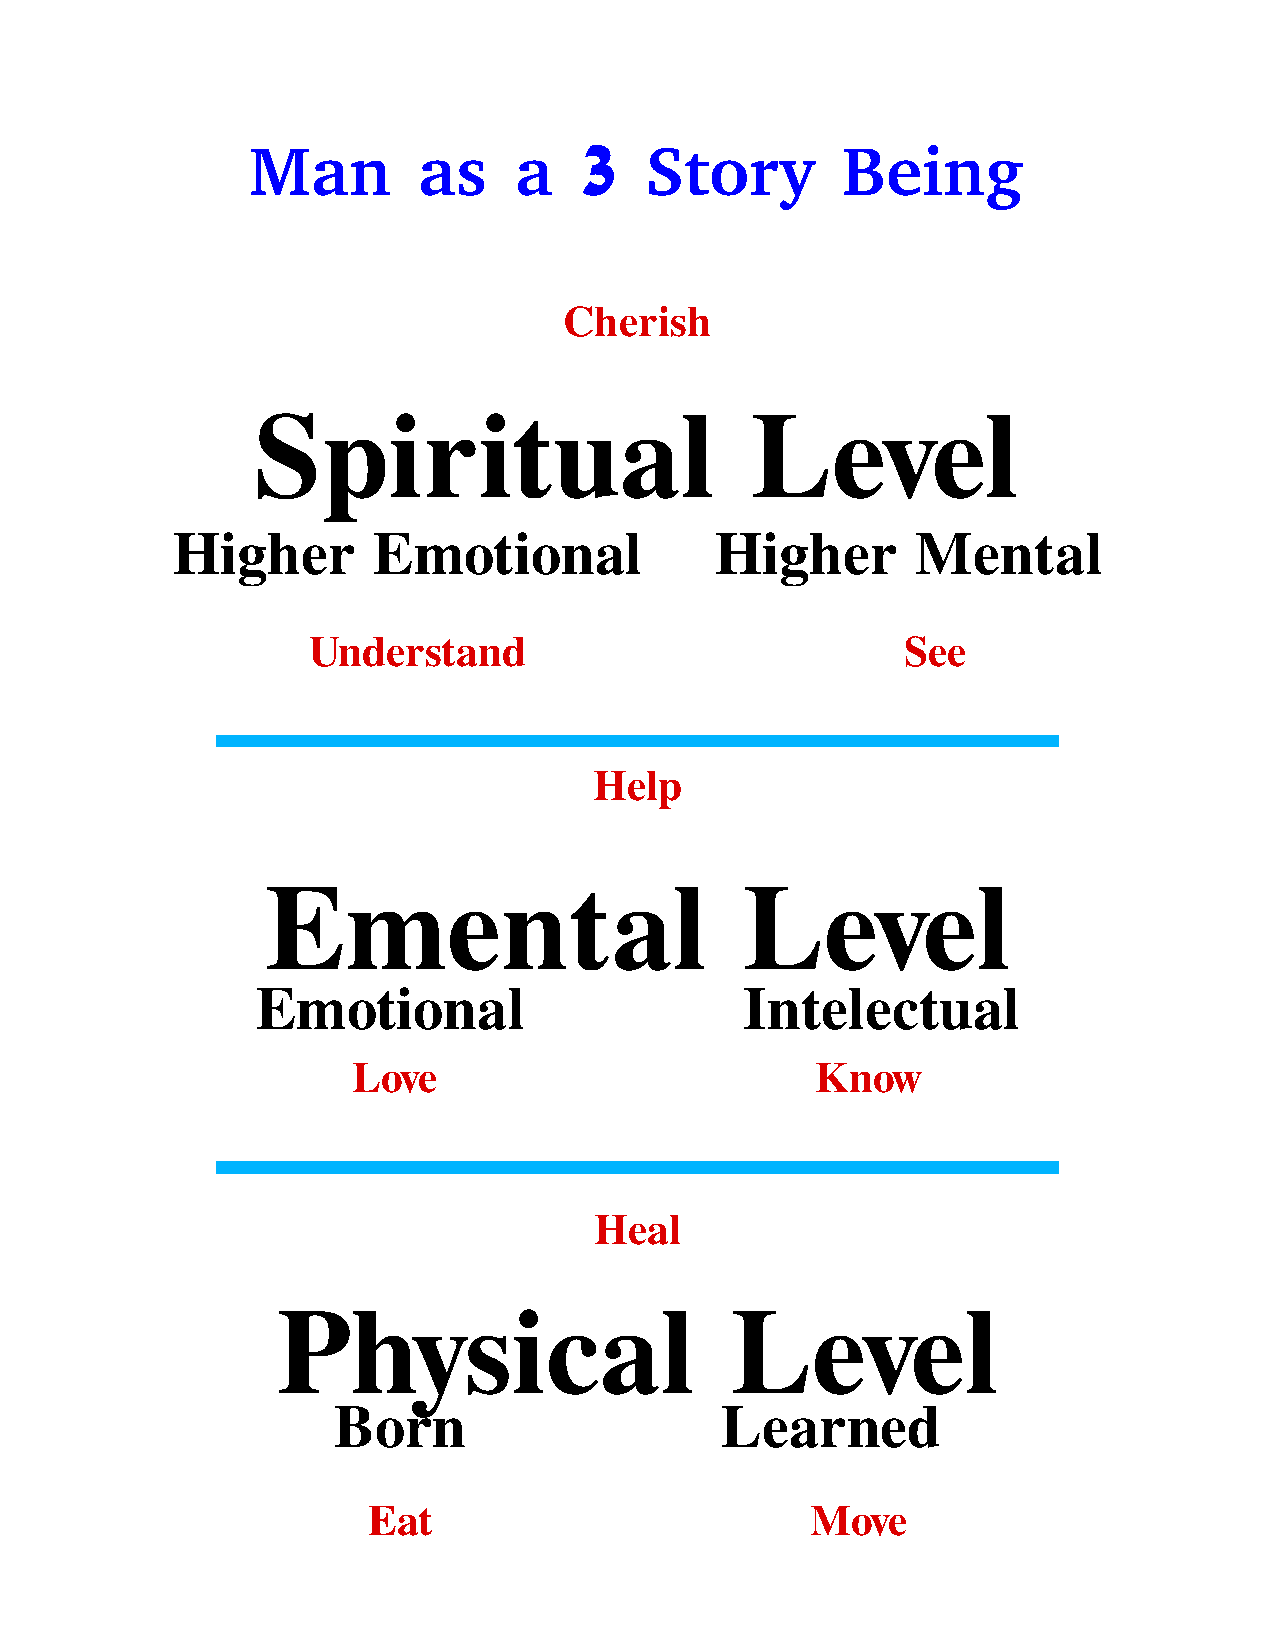
\includepdf[pages=1]{three-story.pdf}
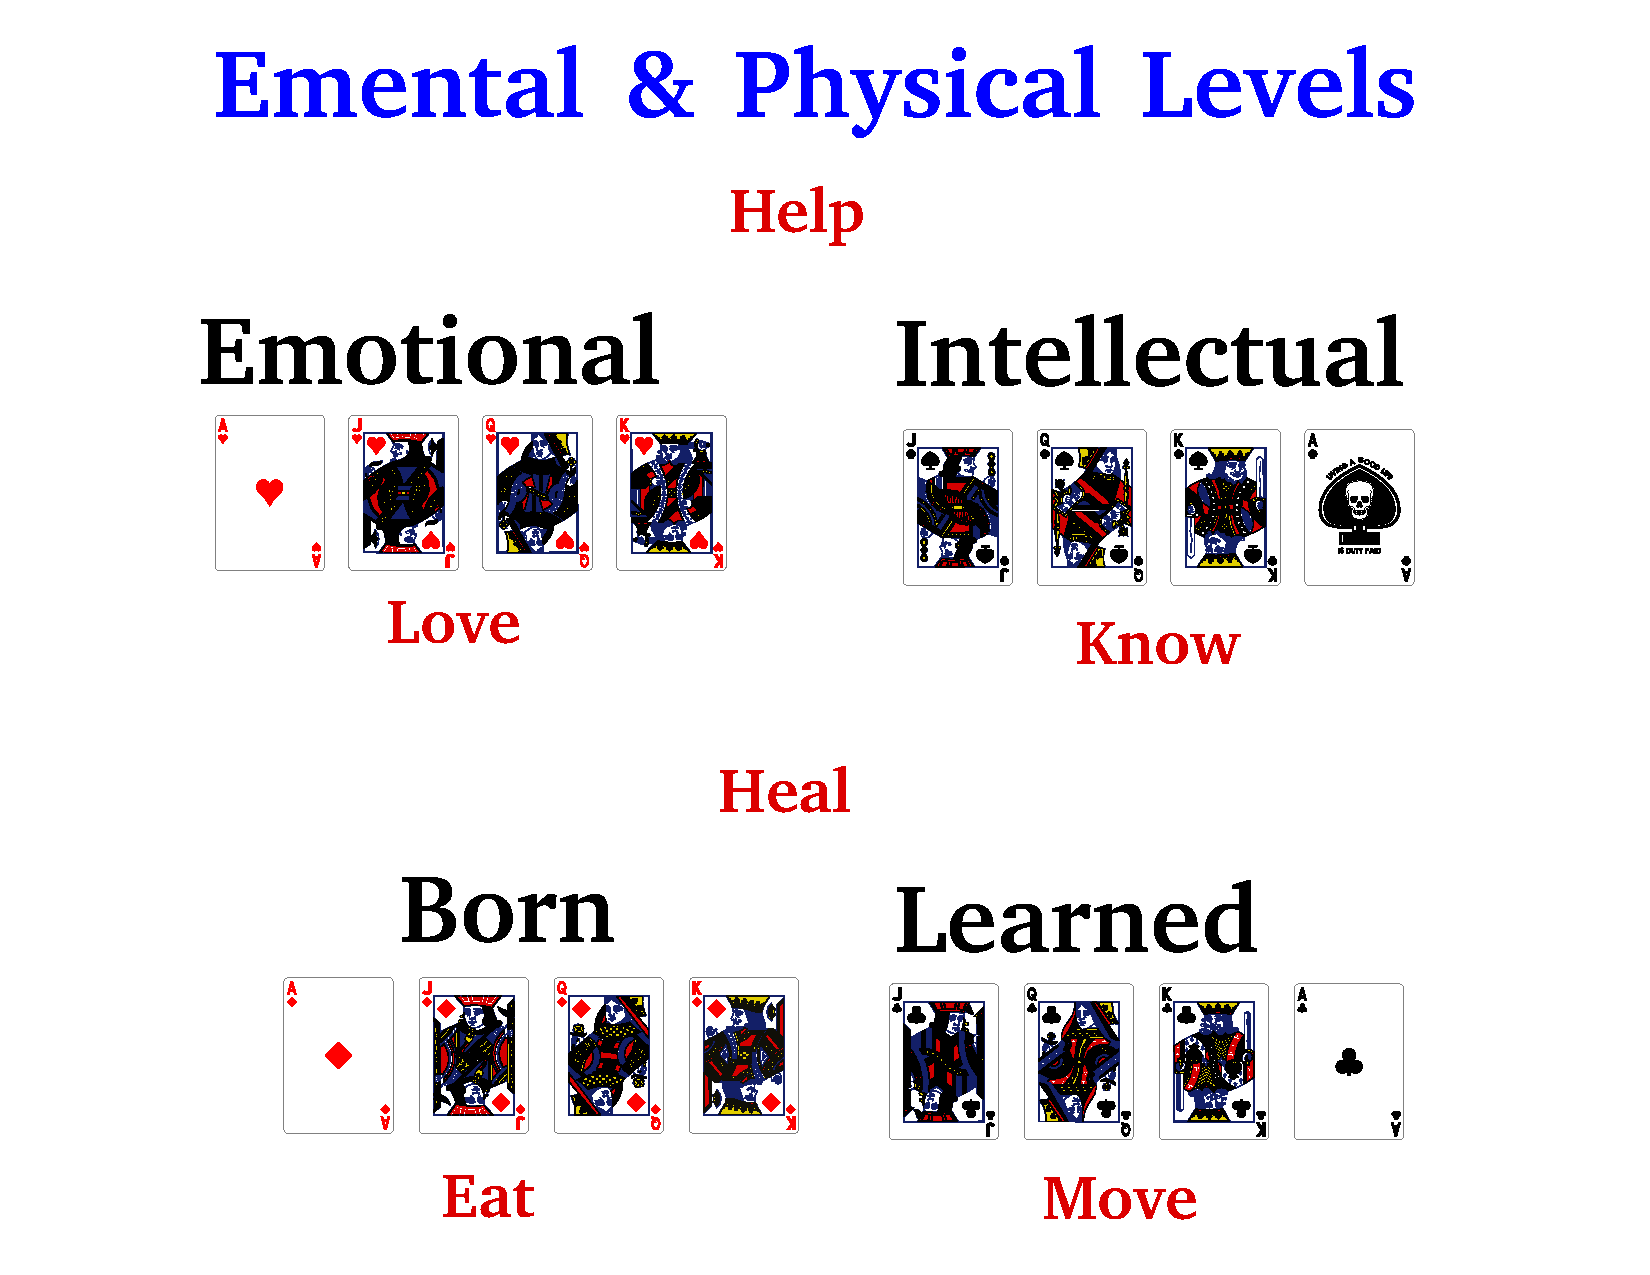
\includepdf[pages=1]{cards-emental-physical.pdf}
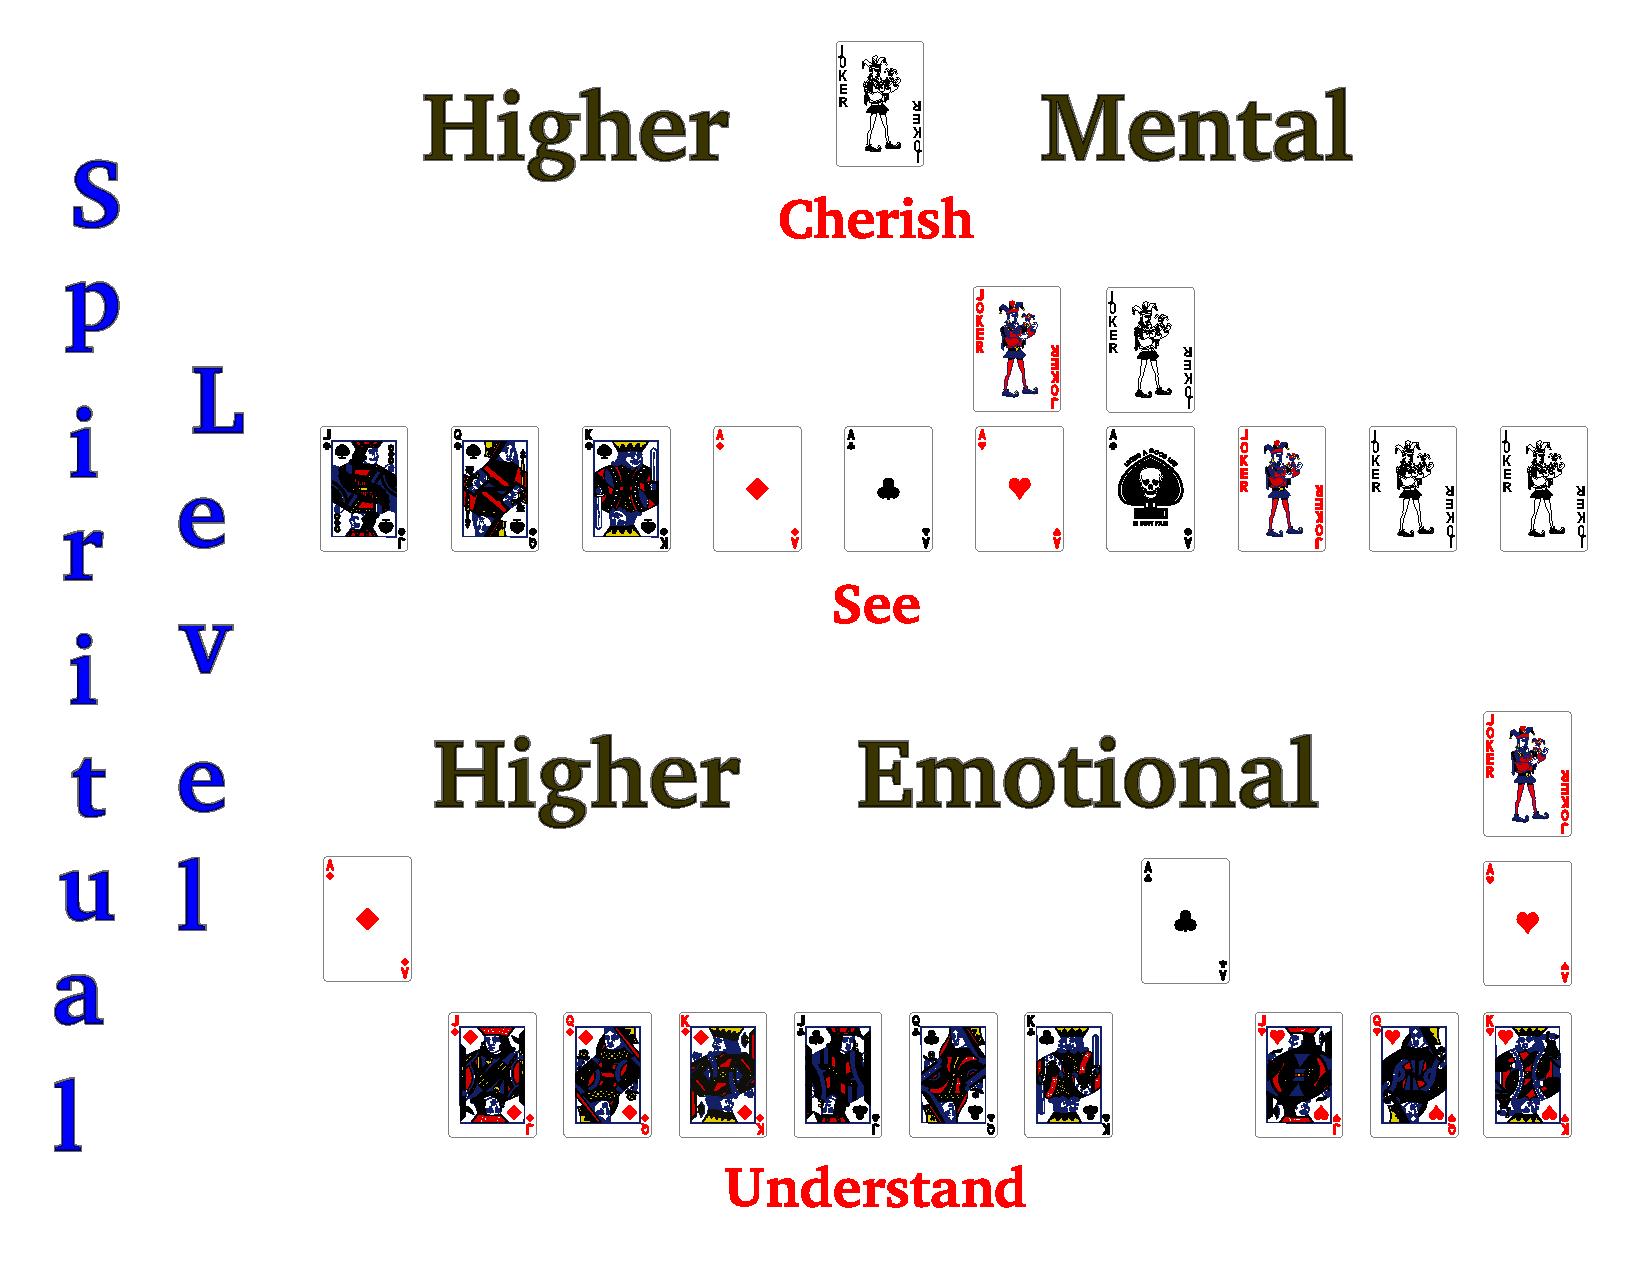
\includepdf[pages=1]{cards-spiritual.pdf}
\chapter{Diagrams}

---

Theese three diagrams, Man as a 3 Story being, Cards Emental and Physical, and Cards Spiritual should always be kept handy. It is good to open them in separate browser tabs on whatever devices you are using. Feel free to print them out if you are so inclined.

---

Man has seven centers: Higher Mental Center, Higher Enotional center, Intellectual Center, Emotional Center, Learned Center, Born Center, and Sex Center. The functioning of higher centers is quite miraculous; and explains why some of Man's ``higher'' moments seem to go beyond the ``sensual-perceived-reality'' of his lower centers. Each center is an independent brain with its own memories, associations, and will. Higher Centers are fully functional but Man, in his present state, has little or no contact with, or control or knowledge of them. Higher centers will function properly if the four lower centers function pproperly. (Born, Learned, Emotional, Intellectual.) The sex center is unique in that it can be thought of as related to our highest spirituality, our our lowest, most base impulses, and everything in between! This is one of the ideas expressed in the four story diagram at the end of this chapter. As we start out in the Games, it is fortunate that we only have four centers with which to concern ourselves: Intellectual, Emotional, Learned, and Born. Understanding what these centers, or brains are, what is wrong with them, and how to fix them is paramount if we want to eventually become fully functional human beings.

Man as a 3 Story Being

This is the main diagram, and the foundation for all that follows. The cards diagrams are expansions of this diagram, adding a huge amount of new knowledge. Note that in the cards Emental \& Physical Levels diagram the two levels of the diagram correspond to the two lowest levels of Man as a 3 Story Being diagram. The cards Spiritual Level diagram, is arranged in two levels to make everything fit on the page, but both levels would sit side by side on the top level of the Man as a 3 Story Being diagram.Our spiritual level is made up of out lower levels, or, to put it another way, our higher centers will be made up of our lower centers when we have perfected our lower centers suficiently. It is not like a light switch, on or off, but a gradual process that proceeds at a rate commensurate with the quantity, quality, and vigor of our efforts! This is a life long endeavor, and we will find things on the Spititual Level that are beyond our wildest dreams!

We have to start our with the physical and emental levels because only by fixing them can we start the process of awakening higher centers. Also, this broken, twisted, and neglected machine is all we have to play with. One of the main objectives of the Games is to help us fix our machines, i. e. our bodies, feelings, and thoughts. It won't take too much studying of the diagrams and ourselvs before we start to understand, a little here, and a little there. And where do you think understanding comes from? That would be the Higher Emotional center! Do you understand, even just a little? You have just made a tiny little bit of progress towards getting your higher centers working better and better. As you progress, you will learn to make larger and larger steps, jumps, leaps, and bounds. You will eventually see that your personal inner (spiritual) journey is not meerly a linear progression, but some kind of geometric or arithmatic progression! 

Let us start on the physical level. On the left side is the born center, which entails everything we are born with. We start life with an amazing machine that does all the stuff that human bodies do. For the most part it just does what it is supposed to do. We see, hear, smell, taste and have the sensation of touch. We don't have to learn to do these things, they're just there and we can use them. We eat food and our bodies metabolize it giving us energy to survive, flourish, and regenerate. Our bodies know how to breathe and regulate our breath so we always have the right amount of oxygen for our current activity level. It is very lucky that we do not have to direct all this from our emental level, because we could not and would quickly die. It is very dangerous to artificially alter some functions such as breathing and heart rate, because its possible that you could permanently damage your body's ability keep itself going. We do, however have some control over our born side. Diet and exercise are the two most important things here. If we give our bodies the wrong fuel, and we all do to some extent, it will cause serious problems on the higher levels. Everyone can probably improve their exercise routines. Most of us need to drastically increase them. Some probably just need some tweaking, and others, such as professional athletes, may need to back down before they permanently damage themselve any more. Lastly are drugs. In our modern society the use of drugs, legal and illegal is rampant. There are no drugs that will help you on your inner journey towards higher centers. The best policy is to eschew all of them, even over the counter pain relievers, to the extent that your medical condition permits.

On the right side of the Physical Level is the Learned center. It contains physical stuff that we have had to learn in our lifetimes. Standing, walking, running, and whatever sports we enjoy operate pretty much automatically, which is a good thing because it would be REALLY inconvenient to have to learn to walk every morning when we wake up. There is also a lot in here which is unnoticed by us and not so good for us, such as jiggling your knee up and down, tapping your fingers, figeting, nail biting, shifting in your seat, and grinding your teeth. This type of manifestation is always connected to negative emotions, and learning to see and control both the physical manifestation and the underlying negative emotions is one of the most important parts of our inner, spiritual path. It is important to note that this center is a LOT faster than our intelectual center. Some people have given the figure 30,000 times faster. There is no way to verify exactly how much faster the learned center is than the intelectual center, but it is pretty easy to see that it is much faster by trying to think out every little motion when you are walking or playing some sport. You can use the intelectual center to analyze a ping pong shot, and figure out how to improve in the future, but if you try to actually do the shot whith the inteletual center, you will lose the game. 

The Emental level has the Emotional center on the left, and the Intellectual center on the right. Notice that the Emotional center is directly above the Born center. This is important because there is a similar relationship between the centers on this level as those on the lowest one. We are born with certain basic emotional functions, and these parts of us more or less function correctly. As we grow up, we learn a lot of negative emental stuff from parents, peers, teachers, media etc. At a very young age children have learned a complex set of negative Emental responses from imitating things in their envirenment. The large majority of this is harmful to ourselves and others and needs to be obliterated. The Intellectual Center is on the right side of the Emental Level, and thinking is much more of a learned thing that emotions. People have to be taught how to think properly. It is easy to see that thoughts and emotions go hand in hand. If we are in a bad mood, we will have bad thoughts; if we are in a good mood we will have happy thoughts. The Emotional center is much faster than the Intellectual center, and it should function even faster than the Learned center. Since our Emotional center is clogged up with so much harmful stuff, it is probably functioning about as fast as the Learned center. This difference in speed makes it very difficult, and often even impossible to use thoughts to stop negative emotions. When that guy cuts you off on the road, that anger springs up immediately and leaves the Intellectual Center in the dust like the Road Runner does to Wile E. Coyote! Besides thinking, the Intellectual center is also in charge of knowledge. Human beings have an incredible, almost limitless, capacity to learn, which is the process of aquiring new knowledge. By learning what is going on inside yourself, and what needs to be changed, you are giving yourself a solid launching point for your own amazing inner (spiritual) odyssey! 

On the Spititual Level the Higher Emotional and Higher Mental centers have a similar born and learned relationsip as on the lower levels. The Higher Emotional center has several properties, dim reflections of which we can see in ourselves and others. It is the seat of understanding,conscience, and the urge to help others, becoming ``we humans'' rather than ``me amoung humans''. This last human trait, is something that, in terms of evolution, was developed in various animals, notably herd animals, as a survival mechanism. %(Interesting to note - couple extra sentences)
Another aspect of the Higher Emotional center is the ability to experience all of our emotions simultaneously. It has been said that if this center was artificially awakened before our lower centers were sufficiently pruified, it could drive us insane. It has also been said that if the Higher Emotional center were somehow opened prematurly, it could freeze all of our negative emotions in us as they are, so that we had no chance of repairing ourselves. Luckily, we have built-in protections which normally keep this from happening. It is necessary to see these sort of reflections, or shadows of Higher Emotional center inside of ourselves and others, but you have to be very, very careful with this. Whenever you see something that you think is a manifestation of higher centers, it always comes with a large dose of egotism, which is something that must be severly, and even brutally limited in ourselves. There is nothing that will stop your inner (spiritual) safari as quickly and thouroughly as thinking you have already arrived. This is something that has been well known since antiquity, but no one has ever really figured out a way around it. Pride, vanity, and egotism are so deeply entrenched in human beings that we must guard against them our whole lifetime! We must be more clever, sly, persistent, and more vigilant than possible to avoid the trap of egotistically thinking that we have finished the journey, or even that we have really made such good progress on it. This is probably the most important single concept that you will ever learn.

Emental and Physical Cards

The fact that common playing cards were designed to show us the inner (spiritual) structure of human beings was ``discovered'' last century by a man who did an intricate and fascinating analysis of musical octaves. Many people feel a fondness for and kinship with the cards from the first time they see them. Is it possible that some parts of us realize they are being talked about, on some levels? Knowing what we are will allow us to see many things in ourselves which had previosly been hidden, which in turn will help point the way along our inner(spiritual) path. The Games are designed to help us grow into the beings we have the right to be. (You have the right not to be negative!) Each center is assigned a suit. Born diamonds, Learned clubs, Emotional hearts, and Intellectual spades. The aces represent the whole center and the jack, queen, and King different parts of the centers. They are differentiated by the type, quality, or quantity of attention operating in the center at any given moment. The lowest part of the center is the jack, which represents the center operating with no attention, just kind of idly ticking along according to whatever random habit patterns it has from copying things in its environment. The queen represents attintion drawn by something outside. The king represents attention purposely directed towards proper inner (spiritual) growth. This is the highest part of the center. Ideally, we want to have a balance of some kind:

``A man should be able to give a total of 30 for everything taken together. This figure can be obtained only if each center can give a certain corresponding number--for instance 12 + 10 + 8

``If 30 is correctly a true manifestation of man and this 30 is produced by three centers in a corresponding correlation, then it is imperative that the centers should be in this correlation.''

There are two ways this applies to the centers. First, it should apply to the Physical, Emotional, and Intellectual, having their proper function in our being as a whole, i.e. Physical, Emotional, and Intellectual being 8, 10, and 12 respectively. In the same way the jack, queen, and king in each center should correspond similarly as parts of each center i.e. jack, queen, king... physical, emotional, intellectual...  8, 10, 12... Don't try to be too litteral and precise about this, the idea is to give us a general idea of how our machine should function, and of the idea that there is a correlation between the machine as a whole and the makeup of each center individually. Let's look at some examples from each center.

The Born center, the diamonds, that with which we are born on the physical level. Our five senses fall into this category. They work primarily with the jack and queen of diamonds. Our senses are always working automatically. This is a good thing because we could not conciously direct them all the time. The born center works at too high of a speed. When an impression comes in to one of the senses, the queen kicks in and our attention is drawn to the sound, movement, change in temperature, smell, or taste. Examples of the king of diamonds could include observing our body and modifying our diet or exercise to improve our health.

The jack in the Learned center, the jack of clubs, includes things like walking, running, and a multitude of big and little things we do every day. These things we do automatically, which is very good and even necessary. Imagine having to stop and relearn all this kind of thing every time we needed it. When learning a new sport, video game, or musical instrument, for example, we are teaching the Learned center. As we progress the queen starts working with the jack to respond to outside events. By practicing movements over and over they become faster and faster and more and more complex. Our Inetllectual center can aid us while learning something new by analyzing some things and giving suggestions after the fact. As our skill level increases, we will start to gain access to the king of clubs. People who get really good at any physical endeavor, will be able to use the king of clubs to do amazing things. A good example of this is great musicians who can create incredible works of art. As we clean up the various parts of our machine, we will gain more and more access to the king of clubs.

The Emotional center, the hearts, is where our biggest problems are concentrated. We exist mostly in the jack, which is constantly flitting here and there following the queen, which is responding to various impressions coming both from outside of us, and also from inside us. We exist as a continuous stream of pleasant and unpleasant emotions. It is important to note that negative emotions, which for the most part need to be disposed of, can be either pleasant or unpleasant. Pleasant and unpleasant emotions come in pairs, for example depression and excitement. One will flip to the other at any time for any or no reason, and we have little or no control over this. Here is a way out: WE NEED TO TRANSFORM BOTH SIDES OF THESE COINS INTO POSITIVE EMOTIONS! Positive emotions cannot exist in the lower centers. They begin in the Higher Emotional center, and are an integral part of the Higher Mental Center. The next diagram, Cards Spiritual Level shows this in exquisite, wonderous detail. There are several ways we can identify positive emotions and separate them from the normal lower emotions which fill our daily lives. Firstly, they do not flip flop into negative emotions. They simply are, and with proper nurturing and prolonged efforts, they will grow, multiply, and expand. Second, they always come with a gift of understanding. This could be about any part of us Physical, Emental, or Spiritual, or about the true nature of things or people in the world. Third, they have a different taste, a particulat flavor which is quite distinct from anything in the lower parts of our being. If we put in right efforts, which is one way to describe the objective of these Games, we will get results. One obstacle that must be overcome, especially in the beginning, is that we do not always get immediate results. Impatience is one of the negative emotions which must be dealt with, and it can present a hard row to hoe! Similarly to the Learned center, by practicing the proper use of the jack and queen of hearts, we will eventually gain the ability to use the king of hearts. Imagine what it would mean if we had full control of our emotions, and were able to direct them to manifest for the good of ourselvs, others, and even the whole world!

The Intellectual center is where we have the most control of all the lower centers. It is by far the slowest of the centers because, as with the other centers, it is not working properly. We, once again, live almost entirely in the jack of spades. One quality of the jack of spades is that it can only count to one or two. Whenever we see things as having only one or two possibilities, we ar almost certainly using the jack of spades. The correct function of the jack of spades is to record, catalog, and organize information, and then hand this over to the queen and king of spades, or any other part of the lower centers as appropriate. The jack of spades should never be answering questions, but only digging up the proper information and handing it on. It is easy to see this in ourselves and others. Whenever there seems to be only one or two options in a situation, it is surly the jack of spades manifesting. (Do you see how the last sentence is a good example of this kind of thinking?) One way to start to get away from this is to come up with at least three possibilities in any given situation. The jack of spades cannot handle three options, so it will be forced to hand it off to the queen of spades and, with enough practice, eventually, to the king of spades as well. Another way to coax the jack of spades to behave better is to give true knowledge which is complex enough that it cannot process it without the help of the queen of spades and the king of spades. These Games are an example of such knowledge. Learning the rules of the Games, the diagrams, and specific techniques for practicing the Games will necessitate that the jack on spades start to step down to its rightful place. As the Intellectual center starts working better and better, it will be able to help us tame the rogue elephant which is our Emotional center.

Spititual Level Cards

This is where the rubber meets the road, where things get really, really fascinating! The two higher centers are made up of almost entirely THE SAME CARDS from the previous diagram, Emental and Physical Cards. The only exception to this is the addition of the two jokers. The Higher Emotional Center is represented by the red erxtra joker, and the Higher Mental Center is represented by the black regular joker. Take some time to look over the whole diagram. You can see that our Higher Emotional Center is composed completely of our Born Center, Learned Center, and Emotional Center. This is why if the lower centers are not working properly the higher centers will not function. You could picture our current state you by imagining that the kings were almost completely removed. This will, of course, be different for various people. Professional athletes and musicians for example will have more development of the king of clubs. The jacks will be tattered and ugly from overuse. The queens will function to some extent, but will be severely under developed. Also notice that the higher centers have the same structure as the lower ones. The three diamonds correspond to the jacks in the lower centers, the three clubs correspond to the queens in the lower centers, and the three hearts correspond to the kings in the lower centers. Our Born, Learned, and Emotional centers in the Higher Emotional center are supposed to have the same 8, 10, 12 relationship in the same way that the jack, queen, and king have in the lower centers. The three acecs, diamonds, clubs, and spades represent the three lower centers as a whole, and the red extra joker represents the Higher Emotional Center as a whole.

The Higher Emotional Center is supposed to be the seat of concience. This is a feature that evolved as a survival mechanism. different species of heard animals survive by putting the welfare of the group ahead of the welfare af any particular member. If  our Higher Emotional Centers were working properly, we would always want to help others in whatever ways and as much as we can. It should be obvious when we look at ourselves and others that this part does not manifest very much or well in the world. Imagine if we could, individually and as a species, lift ourselves up to the levels of cows or goats? Perhaps our species would have a much smaller chance of killing ourselves off through nuclear or conventional wars, hunger, malnutrition, meanness and neglect? Another aspect of the Higher Emotional Center is its speed. It is much faster than the lower centers. If it were going at 30,000 times the speed of the Born and Learned centers, maybe its operation would look simultaneous to our slow lower centers. The Higher Emotional Center is also the seat of understanding. As we fix and tune our lower centers, we will understand many wonderful things. This type of understanding always has an element of positive emotion to it. Positive emotions are the only ones that can exist in the Higher Emotional Center. They do not flip-flop the way emotions do in the Emotonal Center, and they have a distinctive flavor, which we will eventually come to experience, and learn to cherish. The Higher Emotional Center also takes the position of the queen in the Higher Mental Center.

The Higher Mental center is the seat of Reason. It starts off with the perfected Intellectual Center as its lowest part, which corresponds to the jack. The middle part, which corresponds to the queen, is the perfected Higher Emotonal Center. The top part, which corresponds to the king, is made up of the whole of thee Intellectual Center, Higher Emotional Center, and the Higher Mental Center itself. The Higher Mental center is faster still than the Higher Emotional center. It can connect us instantaneously to all the proper knowledge (jack of spades - automatic attention), for the current situation (queen of spades attention drawn by an outside event), and process it all corectly (king of spades intentionally directed attention). It does this so fast that it appears that we make the perfect response without any thought at all. It is fortunate that we don't really have to do anything in the Higher Mental Center, because it is too far away from us in our present state for us to understand very much about it. As we clean up our four lower centers, and start getting the Higher Emotional Center working, the Higher Mental Center will eventually start forming and functioning. It is very important to remember that this center is very far from us in our present state. Being the egotistical creatures we are, it is very easy to fall into the trap of thinking we have already arrived. When this happens our progress along our spiritual path will stop, because why would anyone play Games designed to give us what we think we already have? It is necessary to become VERY familliar with these card diagrams. One way to do this is to start using the cards in our interactions with others. For example, we could say ``When that guy cut me off in traffic my jack and queen of hearts immediately activated, producing some very unseemly emental manifestations.'' When two or more people come together to help each other with the Games (A manifestation of Higher Emotional Center, by the way :-)) what they can accomplish together is a lot more than the sum of what they could accomplish alone. This is probably some kind of an exponential thing. 

All that being said, here is an example of a possible manifestation of Higher Mental center. 25 dollar per game pool.
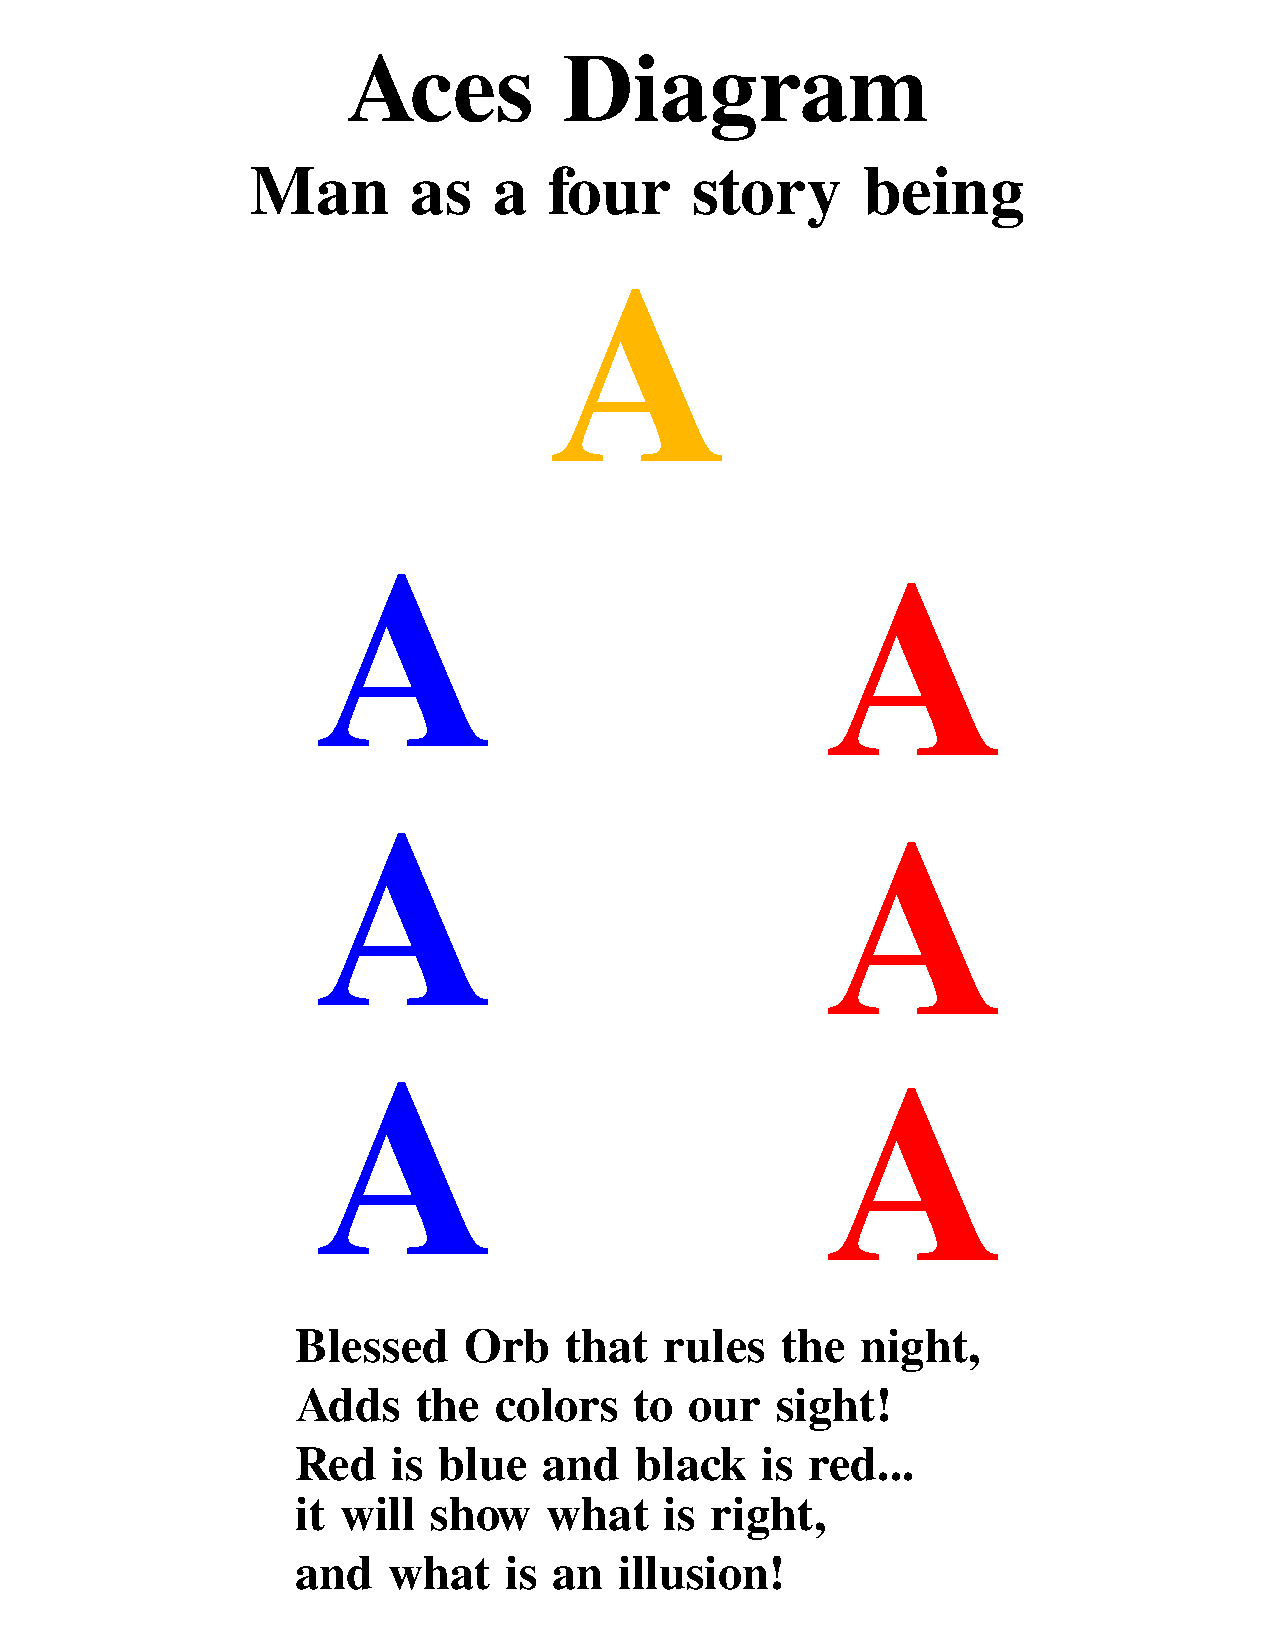
\includepdf[pages=1]{four-story.pdf}
\chapter{Transformation}

The energy expended in active inner work is immediately transformed into new energy; that expended in passive work is lost forever. Whatever you gain through said active inner (spiritual) work can never be lost, it is yours forever. That which is gained through passive work doesn't exist; strangely, and somewhat paradoxically, this makes it extremely difficult to disencumber from oneself.

Think what you feel and feel what you think. Fusion of the two produces another force.

One of the best means for arousing the desire to excel at the games es to realize that you may die at any moment... But first you must learn how to keep it in mind.

In these Games transformation is probably the most important single concept. This primarily refers to transforming negative emotions into positive emotions. So what do you mean, we are supposed to change sadness into happiness, fear into calm, hate into love et cetera? Well, not exactly. All of these, and many more, are what we call pleasant and unpleasant emotions and if you observe yourself and others for a while you will see that this flip flopping is our normal, mechanical state, and exactly that from which we need to escape! These ``normal'' emotions all exist only on the Emental level. What we are aiming to produce through transformation is positive emotions, which can only exist on the spiritual level. We have to start out with the negative emotions because they are the only ones with enough force to drive us to higher levels. By constaltly expressing and indulging in these negative emotions, we are letting the force we need for our inner (spiritual) journey leak away and dissipate. In order to have the force to create the positive emotions which will drive the growth of out Higher Emotional center, we must observe our negative emotions, avoid expressing them, and use all of our wit and cunning to go against them.

So let's start out by looking at the Emental Level on the cards diagram. The aces represent the center as a whole, and the jack, queen, and king are the three parts of each center. Each center has its own memory, associations, and will, which correspond to the jack, queen, and king respecively. The parts of the centers can also be recognized by the type of attention involved in it's operation. The jack needs no attention, it functions automatically. The queen uses what is called drawn attention, that is, the attention is drawn by some outside object. The king represents directed attention, or will, which always requires an intentional effort on our part. We don't use the kings very much, and they are key to transformation. The jack and queen alone will leave us flip flopping as we always do, it takes no effort to let our jacks merrily(or more often sadly and bitterly) go their way, while whatever external events are around us cause our attention to go hither, thither, and yon! It is only by using the will, represented by the king, and also known as effort, to go against our negative emotions that we can drive our inner (spiritual) journey forward.

Since the aces are made up of the jack, queen, and king of the suit, we will examine only the three cards, the jacks through kings, in each center. The jack of hearts is responsible for emotional memories. We all have plenty of these which can be pulled up at any time by anything which happens to pass into our lives. We can also recognize the jack by seeing how our emotions flit around here and there all by themselves, as when daydreaming or just sitting quietly. The queen is a little more complex. Whenever anything comes into our attention, we will immediately have some kind of emotions about it. We like this, we don't like that, we are afraid of this, but that makes us feel safe, we are bored by this, excited by that, angered by this, enamoured by that. This shows the action of the queen of hearts in the sense of it being drawn attention, i.e. drawn by an outside object, and also in terms of its property of associations. Whatever comes within our percetion, we have an immediate and automatic response to it. The jack and queen of hearts can only act mechanically, that is without any will or effort. So what would the king of hearts entail? It would mean that we had used will, or effort, to produce whatever emotion we wanted to. Everyone has a little of this, i.e. can you act happy around your boss, or an important business contact? Most of us are probably not really so good at this, often being quite transparent to those we are trying to fool. For others, this type of business behavior is well ensconced in the queen of hearts, so there is no effort involved. Some great actors probably also have a bit of the king of hearts, but in everyday life they may not do any better than the rest of us. For the most part our emotional centers are out of our control, like a rouge elephant dashing here and there breaking and hurting things, mostly ourselves. So we must find a couple of elephants we can control better, and get them onto the job!

The first tame elephant at our disposal is the Intellectual center. The jack, once again, has to do with memory and works auromatically. This, in itself, is not a bad thing. The job of the jack is to take in impressions, keep track of them, and send them out to the appropriate place when needed. The jack of spades should not only be sending the appropriate memories and incoming impressions to the queen and king of spades, but to the other centers also as it is appropriate to do so. The jack of spades should never respond for us, but this is pretty much all that ever happens. This is quite easy to observe in ourselves and others. One characteristic of the jack of spades is that it can only count up to two. This is binary thinking and it is easy to see all around us. (Look on any social media!) This binary thinking is a prerequisite for all kinds of negative emotions. Note that when someone says that there is only one way to look at something, or one thing to do, he really means that there are two, and yours is wrong. This is the main idea behind the many ends of the stick Game. If you give the jack of spades more than two things at once, it may start working more normally, and stop shouting the same thing over and over. Of course the jack of spades is almost always in cahoots with the Queen of spades, which is in charge of all the myriad associations between what the jack of spades has collected and is collecting. The Queen of spades is drawn to whatever impressions are around us. Some impressions will tend to lift us up, and others will tend to bring us to our lowest levels. It would behoove us all to ponder this VERY, VERY carefully, for it is one area in our lives where we can have a significant amount of control. Do you want to go watch a horror movie, or study and contemplate the Games diagrams?

Our primany aim is to transform negative emotions. The basic technique for doing this is to use intentional effort to change them at any given moment. First, we have to notice that we have negative emotions, and realize that they are bad and need to go away. How many times have you seen someong say ``I'm not angry!'' very angrily. This is an indication of what is called a buffer, which keeps us from seeing unpleasant things about ourselves. A person with such a buffer can run around all day being angry and snapping at people and sincerely believe that they do not get angry. One very effecive method for finding and seeing buffers in ourselves, is to look at which manifestations of others really bug the heck out of us. The limits of our ability to endure the manifestations of others will show us very important things about ourselves, i.e. they may point the way towards our buffers. It is very important to have others around us for the Games, and this is one example of why this is so important and useful. Others can show us today what it might take years or decades for us to figure out on our own, and life is short, so there are certainly many things that we just would never have time to get to on our own. Once you start to glimps the incredible wonder and limitless heights possible on your inner (Spirtitual) walkabout, it may give you a proverbial kick to get you off the proverbial ground.

There was once a young man who encountered these ideas in his early twenties and was immediately enamored of them. He was a very angry young man, and it was easy for him to immediately see this. He was also immediately amazed that here was a completely brand new idea, i. e. that negative emotions like anger were bad and needed to be gotten rid of. However, it never occured to him that he was a mean person, and if you would have asked him if he was, he would have denied it. So, this angry young man, with the help of some very dear and intelligent friends, worked literally for decades trying to go against his anger, and bit by bit he made a good bit of progress. Then, at a certain point in time when he was already an old man, he finally progressed enough to see his meanness, and one day it pretty much all came barrelling down on him all at once. This is an example of God, or Higher Centers, or Nature not letting us see things about ourselves until we are ready to see them. So what happened to the guy? Well, due to the eforts this man had made against his anger, and many other similar efforts, he was not horrified, shocked, or even particularly surprised. He kind of felt, oh, I wonder why I never saw that before, while at the same time knowing full well why he had not. And with all his prior efforts it did not need decades to deal with these new revelations, but he continues progressing, seeing and transforming things every day! The angry young man had always hated mean people intensly. Once you see something in yourself, and rest assured, you have everything in yourself, you will easily see it in others, and also easily endure others' manifestations of said something.

You may be asking, so if the angry young man saw the meanness in others, and so did the much less angry old man, then what's the difference, didn't they both see the same things? Here is a very wonderful thing to know and understand. The angry young man saw people's meanness through the lens of the Emental Level, which has things like self pride, vanity, anger, negative emotional judgement, fear, negative imagination, and many other things unbecoming a human being all mixed up in things. The much less angry old man saw  it much more through the lens of the higher centers, where all of these things cannot exist. On the Emental Level, you get a very binary, and rough tasting approximation of a situation. Through the lens of higher centers, you see many different truths on many different levels, and you see it all at once. It is a much different taste, and it does not evoke any negative emotions in the person experiencing it. Like all things spiritual (inner) this is not a yes or no thing, but a process that starts when you start cleaning and fixing up your inner machine. As you progress, you will be able to start to tell the difference between things coming from higher and lower places in yourself, and it will help guide you on your journey.

It is also worth noting that while the old man had indeed made quite a bit of progress, he still has plenty of inexactitudes left on his Emental Level to keep him busy, day to day, for the rest of his lifetime.

The second tame elephant is our body, and everyone has a certain amount of control over it. Our body is represented by two centers on the lower story, the born and learned centers. They are so named because these name remind us how to properly see the different functions in our bodies. Our five senses are things that everyone is brorn with, as are our basic bodily functions such as digestion, growth, and regeneration. On the Learned side, we can walk, run, ride a bycicle, play foozball, etc, all the things we have learned to do with our bodies throughout our lives. There is also much that can potentially be gained by learning new physical activities while looking at the preocess through the knowledge of the Games and Game diagrams. We can put in useful efforts here though improving diet and exercise, and every effort made with the intention of helping us along our spiritual (inner) journey, will be a manifestation of one or both kings on the physical level, either that of diamonds, clubs, or both! Several of the Games include efforts to make us aware of and give us control of our bodies. When the rogue elephant that is our emotional center is lashing out and overpowering our intellectual center, we may be able to bring in the body to tip the balance.  

At this point we can summarize some ideas about our inner oddessey. In order to commence and propel us along our amazing personal path, we need will, or effort from all of the four lower centers, which is represented by the four kings, diamonds for Born, clubs for Learned, hearts for Emotional, and spades for Intellectual. The centers are all interconnected in myriad ways, much being good and useful, and so things that we want to strengthen, clean up, and encourage to grow. Most of our problems are centered around negative emotions, and many things especially in the Intellectual center, but also in the Learned and Born centers, which contain many bad habits, and damage from whatever we have been through in our lives. One ally that is much more than we realize is our attention. Each center has it's own attention, and we can learn to use the different attentions we have to learn about our machines, and even start to aise our attentions towards higher levels, spiritual levels where our true home awaits our return!

Emotional fear vs Born fear

Fear in the Emotional Center is mostly a very bad thing, which causes all kinds of Emental problems. It is possible to learn to discern these two kinds of fear and maybe some examples need to go here? cross the road at any time without looking.
A. You speak about instinctive fear; emotional fear is different, it is based
on imagination.


 All our life, all our habitual ways of thinking, have only one
aim—to avoid shocks, unpleasant feelings, unpleasant realizations about ourselves.

Curiosity is a special emotion which exists in each centre. In the intellectual centre
it is connected with desire to know.

But this refers only to intellectual attitudes. In emotional centre, negative emotional attitudes mean identifying.

 trying not to identify is the best means of passing into higher parts of centres. 

Negative emotions, can be either pleasant or unpleasant, and this can be very different from person to person, and can even change for a certain person according to the situation.

fear anger bored meanness guilt feeling sorry for yourself(internal considering vs external considering) greediness unhappy dissapointed dislike pity 

%\chapter{Emental and Physical Levels Cards Diagram}
%\chapter{Spiritual level Cards Diagram}
%\chapter{Four Story Diagram}
\chapter{Games}
\section{The Basic Games}

oot/oat

red words game

Every time you gain a little knowledge and understanding your ability to love and appreciate progress on your inner path will increase. The higher (understanding) blends with the lower (knowledge) in order to actualize the middle (king of hearts) and thus becomes either higher (king of hearts) for the preceeding lower (knowledge) or lower (king of hearts) for the suceeding higher (understanding). 


reminding factors

\section{Intellectual Games}

many ends of the stick

Related Associations Game from chapter 2 vvov.

memorize game

\section{Emotional Games}

Related Associations Game from chapter 2 vvov.

the blame game

\section{Learned Games}

mechanical movement

\section{Born Games}

Pay attention to your breath while you eat game.

Pay attention to every part of breath in every bite of every meal. Bites include drinks too.

This is one of the most important games. It offers a unique opportunity to bring in the second elephant to help reign in the rogue elephant which are the jack and queen of hearts.
The diamonds represent what we are born with, and eating is probably the most masic bodily function over which we have some control. Remember that control, when used with the intent to guide you along your own, personal, inner (spiritual) path is a manifestation of the king of the cente, in this case the king of diamonds.
The king of spades, which you are exercising ritht now by learning, studying, and practicing these Games, helps the diamonds and clubs to reign in the jack and queen of hearts.
We have been eating since no more that a few days after our births, so it is easy to imagine that this might be a very strong part of ourselves. There is a very interesting and powerful form of identification involved in eating, which can sometimes be observed if you see someone eating without practicing table manners.
When you see this you will be reminded of a wolf devouring its prey, and it is ugly, primal, and a bit scary. At some point you will be able to learn to see this in yourself, but you will most likely have to practice this game for a while before being able to do so.
It might also be possible to see this clearly if you take videos of yourself eating when you are alone and very hungry.

It is also not so easy for some people to actually do this Game. There was once an hour long meeting of a group of ``spiritual Masters'' who sat around for the whole hour commiserating about how hard this Game was.
Not one of them had actually ever been able to remember to try it. If you are in this category then there is probably no hope for you whatsoever, and you may as well just give up on the Games without going any further.
There is no point in having someone who is so weak that they can not even start to practice this simple game go forward.
There is no path open to them. On the other hand, its going to take a lot of effort and perseverence to follow and progress on your journey, so this is a perfect place to make a stand, and do whatever it takes to get into this very good pattern of behavior.
One very good way to do this could be to use reminding factors.
For example, switch your watch to the other hand, so that when you look at the watchless hand to see if its lunch time, it reminds you that you need to remember to pay attention to your breath when eating. Perhaps you could buy yourself a new piece of jewelry just for this purpose, whenever you see the item, you try to remember this Game.
Or maybe writh WATCH BREATH on the front or back of your hand. Or maybe you could bring in the first tame elephant, the king of spades. Make up a poem called Watch My Breath, neither too short nor too long, and memorize it.
Your lunch break is the perfect time to play at memorization, and if your poem is about watching your breath, it seems likely that you may be able to actually do it during lunch. Now here is one that only the woemen, who generally have better developed jacks and queens of hearts, can try: bring in an emotional element to the poem, make it about a magical unicorn, frolicing fairies, or a beautiful butterfly, and then share it with some men, they can probably catch up eventually!

Once you actually get started with this Game, there is a lot more there to see and do than one might imagine. First of all, can you actually perform the game according to the basic rule: Pay attention to every part of breath in every bite of every meal. This means inhale and exhale. Its best to start of when you are alone. Move to an empty table, go to a secluded place, or an empty room to eat. In the beginning it wil probably be impossible to play this game while in the company of others, unless they are also playing the Games, which is the best situation of all! What about eating different things? A piece of hard candy (NO BITING) will take a whole lot of breaths. If you are eating a piece of meat which needs chewing, probably a few breaths. Drinking a mouthful of water? Seems like one or two, depending on whether you count in and out as one cycle or two breaths. It is important to note that you should never try to change your breathing, because it could cause permanent damage. Your jack and queen of diamonds, your body, knows how much you need to breath in any given situation. Let it do its job, you can't do it properly, and you certainly don't want to have to. It is also good to bring in the other centers here. You can observe with the jack and queen of spades how various foods affect your tummy. Most of the food you eat will have a bad effect on you, and whem you notice this you can, if you remember, eat something else next time. Of course the jack and queen of hearts are always good to invite to the party. Did you know that around a third (33\%) of the world's population suffers from hunger? That should be enough to make even the jack and queen of hearts challenged men feel a little grateful while they are scarfing down their vending machine tuna salad sandwitches! Actually, and pleasant emotoin (Emental Level) which has the potential to be transformed into a positive emotion (Spititual Level) will work, and the strongerthe pleasant emotion the better. Remember also that in the Games rewards are not always immediate. Sustained efforts, which represent the kings of the centers, repeated over time will kind of build up, leading to really wondrous revelations in the future. This also relates to the idea of ``Like what it does not like.'' If at any moment we do what the machine is accustomed and likes to do, it is the jack and queen of the center, the energy used is lost forever, and we remain stuck in our normal mood swings. However, if we intentionally go against all this normal stuff, the machine will be uncomfortable, it wants to keep everything as it is. By exercising and practicing the kings of the center, we can save energy, a little here and a little there, and eventually get the Higher Emotional center to start working. This is where we can start to glimps positive emotions, which always come with increased uderstanding, more and more finely tuned knowledge, and a drawing closer to whatever conception of God you currently have. You can only really know, understand, and get closer to God on the Spiritual Level, and you will be amazed at the things you will encounter on your own, personal, inner (spiritual) journey! 


%even meanness has its place and usefulness, see second paragraph above

lying still

\section{Sexual Energy Games}

I know why I don't go to extremes extremes game gurdjieff abuse and use of sex

\section{Miscellaneous Games}

What do I call identification (identifying) and how and where do I describe it?

binary thinking I never argue, buffers.

buffer game

\section{Song Games}

So, if one had a story to tell, which was actually an alegory, and wanted to tell it in a  pop music style song, one could come up with several choruses, which conveyed the central, most important ideas/concepts, and then lead the listener through the story by presenting the verses in a progression, perhaps through time, perhaps even through dimensions above time, and put real, understandable examples in the verses, and them put the choruses in as appropriate to emphasize a point in a verse, transition to the next verse, or point out a fallacy in a verse.

    Think of it like a plot twist in a story: the chorus is your thesis, the verses are the examples, and the bridge is the “aha moment” that makes everything click.
    
    
Go to Extremes Parody

[Verse 1]
Call me a joker, call me a fool
Right at this moment I'm totally cool

Clear as a crystal, sharp as a knife
I feel like I'm in the prime of my life

Sometimes it feels like I'm going too fast
I don't know how long
This feeling will last

Maybe it's only tonight

Call me a joker, call me a sinner make sure you never call me late for dinner

Everyone yearns for happy endings. We need to learn to find happy beginnings. And they are more and better than you can imagine!!!

[Chorus 1]

Darling I know I should not go to extremes
Too high or too low I must stay in between
And while I stand fall and play the middle's where I need to stay
Darling I know I should not go to extremes

[Verse 2]
Sometimes I'm tired, sometimes I'm shot
Sometimes I don't know
How much more I've got

Maybe I'm headed over the hill
Maybe I've set myself up for the kill

Tell me how much
Do you think you can take

Until the heart in you
Is starting to break?

Sometimes it feels like it will

[Chorus 2]
Darling, I don't know
Why I go to extremes
Too high or too low

There ain't no in-betweens

You can be sure when I'm gone
I won't be out there too long

Darling, I don't know
Why I go to extremes

Extremes take the edge off of your play Energy there makes your games go astray

Follow the path of your life embrace all the fun and the strife

Darling you must stay away from those extremes

[Verse 3]
Out of the darkness, into the light
Leaving the scene of the crime

Either I'm wrong
Or I'm perfectly right every time

Sometimes I lie awake, night after night
Coming apart at the seams

Eager to please, ready to fight
Why do I go to extremes?

[Bridge]
And if I stand or I fall
It's all or nothing at all

Darling, I don't know
Why I go to extremes

[Chorus 3]
Oh, I don't know
Why I go to extremes

Too high or too low
There ain't no in-betweens

You can be sure when I'm gone
I won't be out there too long

Darling, I don't know
Why I go to extremes

[Outro]
I don't know why, I don't know why
I don't know why, I don't know why
I don't know why, I don't know why
Out of the dark, into the lights
Whether I'm wrong, perfectly right
I don't know why


I simply practiced what Gurdjieff suggested. Here, I won’t list all my arsenals, but a few … to review ideas. I observe myself alone, I observe myself with others while keeping the face and the eyes alive as G advised; I observe my postures, my responses, my mechanicalness, etc. I keep vigilance for leaks; double-check for illusion; watch ego; flag internal considering; monitor thoughts, attitude, attention, and atmosphere, etc. Practice not doing as others do, taking the eight, taking the blame, listening – which is different than hearing. Remembering not to contribute to others’ sleep, not to call a man a slug. Question if it is real I, or some little clever biased I in the driver’s seat, question my accuracy. I experiment with influences using different tactics to see which works best, and, as Gurdjieff said, if one doesn’t work, try the other

Laughter enters my Purgatory forever. Realizing the ludicrous situation of what I had become due to life circumstances and influences…that there really was no me…just remnants of poisoned impressions creating this glob of hypnotized, unaware, chemical robotic machinery that could not even think for itself, had no independence, and was buffered out in illusory perceptions…well, thanks to freedom, that simply made me laugh. I now laugh at all the parts I have not died to. Laughter dwells in my Purgatory


%understanding, seeing and cherishing are ways of verifying that exist on the spiritual level.
\chapter{Sayings}
* Like what it does not like.

We must destroy our buffers. Children have none; therefore we must become like little children.

It is very useful to try to find what buffers are. Try to find how one lies to oneself
with the help of buffers. Suppose one says 'I never argue'. Then, if one really has a
good conviction that one never argues, one can argue as much as one likes and never
notice it. This is the result of a buffer. If one has a certain number of good buffers, one
is quite safe from unpleasant contradictions. Buffers are quite mechanical; a buffer is
like a wooden thing, it does not adapt, but it plays its part very well: it prevents one
seeing contradictions.

We attract forces according to our being.

One twentieth of all our energy goes to emotional and instinctive centres. Self-remembering is a lamp which must be kept alight by energy from these two centres. Our thinking centre is not really a centre, but an apparatus for collecting impressions.

We have good and bad angels. The good angels work by way of our voluntary, active nature and the bad through our passive nature.The Amanon are the good angles.

Mr. Self-love and Madame Vanity are the two chief agents of the devil.

Do not be affected by externals. In themselves they are harmless; it is we who allow ourselves to be hurt by them.

We never reach the limits of our strength.

If we do what we like doing, we are immediately rewarded by the pleasure of doing it. If we do what we don’t like doing the reward must come later. It is a mathematical law and all life is mathematics.

Men have their minds and women their feelings more highly developed. Either alone can give nothing. Think what you feel and feel what you think. Fusion of the two produces another force.

An ordinary man has no ‘Master.’ He is ruled now by the mind, now by the feelings and now by the body. Often the order comes from the automatic apparatus and still more often he is ordered about by the sex centre. Real will can only be when one ‘I’ rules, when there is a ‘master’ in the house.

You should forget about morality. Conversations about morality are simply empty talk. Your aim is inner morality.

To gain anything real, long practice is necessary. Try to accomplish very small things first.

To bear the manifestation of others is a big thing. The last thing for a man.

In the river of life suffering is not intentional. In conscious life suffering is intentional and of great value. 

The highest that a man can attain is to master the Games.

The worse the conditions of life, the more productive the Games, as long as you learn, remember and play them.

Oot/Oat always and everywhere.

Remember that the Games are for struggling with yourself and only yourself... So thank everyone who gives you the opportunity.

Here we direct, create conditions, and help. Be sure to remember this and always treat others accordingly!

* Know that this house can be useful only to those who have recognized their nothingness and wh believe in the possibilith of changing.

If you already know it is bad and do it, you will not succeed very much in the Games.

The chief means of happiness in this life is the ability to always consider how to help others first and yourself second, until you advance far enough to realize that you don't have to choose.

* A true sign of a good man is if he loves his father and mother.

* Do not love art with your feelings.

* A true sign of a good man is if he loves his father and mother.

* Judge others by yourself and you will rarely be mistaken.

Help everyone who is playing the Games, or willing to.

* Respect every religion.

Respect those who put GREAT effort into the Games and make every effort to help them.

* We can only strive to be able to be christians.

* Don't judge a man by the tales of others.

* Consider what people think of you, not what they say.

* Take the understanding of the East and the knowledge of the West, and then seek.

* Only he that can take care of what belongs to others may have his own.

* Only concious suffering has any sense.

* It is better to be temporarily an egoist than never to be just.

* Practice love first on animals, they are more sensitive.

* By teaching others you will learn yourself.

Remember that the games are not for their own sake, but only a way to advance you along your unique path.

You can only be fair to others to the extent that you can put yourself in their place.

* If you have not by nature a critical mind, your staying here is usless.

He who has freed himself from the disease of ``tomorow'' has a chance to excel at the Games.

Blessed are those who are far advanced in the Games, and blessed are those that have never heard of them, but woe and grief to those just struggling to start out in them.

* Rest comes not from the quantity but from the quality of sleep.

* Sleep little without regret.

One of the best means for arousing the desire to excel at the games es to realize that you may die at every moment... But first you must learn how to keep it in mind.

Spiritual love evokes the same in response, Emotional (Emental?) love evokes the opposite. Physical love should never be used for extortion, kidknapping, robery, etc.

Spiritual faith is freedom. Emotional (Emental?) faith is slavery. Mechanical (physical) faith is foolishness.

* Hope, when bold, is strength. Hope with doubt, is cowardice. Hope with fear is weakness. 
Bold, Spiritual hope is strength. Hope with negative emotions such as anger, fear, doubt, jealousy, or boredom is weakness, cowardice, and ???.

* Man is given a definite number of experiences--economizing them, he prolongs his life.

Here there are neither Russians nor English, Jews nor Christians, but only those who persue one aim--to be able to play the games.

* Where there is more, more is added; where there is little, even that is taken away.
Christian parables

Freedom is a stick with many, many ends.

* Self initiation menns never having to blame someone else for your lack of progress.

* People have the remarkable ability to major in minor things.

When your knowledge of the Games becomes the language of your mouth and the basis for your actions, you will understand.

* Maintaining sleep is a tacit conspiricy.

There is always a Game or three you can play.

* A sleeping man will be able to constate the moments he was concious; a concious man will be able to constate the moments he was asleep!

Game knowledge of things you have not yet fully accomplished on your unique life path will be as seen through a glass darkly.

Games are not going to make us, but by playing them hard and well we can make ourselves.

Be wary of asking permission to help another.

Sometimes you can see the shoes someone else is wearing, sometimes you can see your own, accomplishing either one can help with the other. When you have two or more people looking at the shoes, amazing things can be done.

Recognizing that you do not know is one of the greatest momnents of knowing.

* Understanding trumps knowledge.

* Sacred cows function best if fed -- or slaughtered.

* What a man sees when he looks at the world around him says more about the man than it does about the world.

Spiritual truths often get lost in the minutae of definition.

To be or not to be may be the question; but to be and not to be is the answer.
\chapter{Crystal Vision}

Amanon

Car girl, pichones

Fish in house on hill, geese in dry lake which eat the fish and mushroom like things growing around in lake

violent dream after reading pamela's purgatory: driving areund in van with evil passenger going to some important event that he wants to keep me from. one person that I wanted to help has left back of van from early in dream, one other is still there with some phones and other gadgets, but not doing much. pov is driver passenger probably same person, guess who?

\chapter{The Perfect Diet aka Anti SAD Food Diet}

This part is referring to food in the USA, but it seems likely that the situation is similar other places. The parts about starting points in order to find your perfect diet should be feasable anywhere, and may even be easier to implement in ``less developed'' countries.

Well, in this chapter we can hear out astute readers ears perking up and asking ``The perfect diet? Do you really think you can fond one diet that works for everyone?'' And the answer to this question, of course, is no. What we are outlining here is, however a diet that anone can try and eventually figure out what her exact, perfect diet consists of on any given day. In order to do this it will be necessary to fine tune the human machine on the Physical, Emental, and Spiritual levels. Pretty much all of the food that you eat makes you sick in one way or another. In this regard, food can be divided into two broad categories, food that is spoiled, or rotten, and food that is not fit for human consumption in th first place. Much of your diet probably consists of foods that fit into both categories. This causes huge problems for anyone trying to advance along their own, personal, inner (spiritual) path. When there is a problem in the born level, such as when one consumes spoiled or inappropriate food, the whole organism functions poorly. (Have the card diagrams handy.) It should be obvious that problems in the jack and queen of diamonds, the born center, it will be likely to affect the learned center, jack and queen of spades, the learned center. If you are sick, you are not going to be able to walk, run, or play sports optimally. These two centers are on the same level, the physical, so it's kind of obvious that they will be closely linked. If you are very skilled at any physical endeavor, playing pool for example, you may be able to notice that if your stomach is upset, you can notr peform at the peak of your ability. The same kinds of things can be seen on the Emental livel. If your stomach is upset or your gut is aching, you will probable be in a bad mood and thiking bad thoughts. This is something that everyone should be able to see, both in themselves and in others. This type of observation is very useful and important in the Games. One way of looking at it is that your ability to engage the king of the center is impaired or absent. Our ability to engage the kings of the centers, which represent concious effort with the purpose of progressing on our inner (spiritual) journey is paramount. Without the kings we can never reach the Spiritual level, and if one or more are damaged or debilitated, whatever contact with the Spiritual level we manage to gain, will be less than it could be.

One important food item is meat, and many people have various thoughts and opinions on this topic; a fair number of these have decided not to eat meat. They may have noticed that eating meat makes them sick, which is because all the meat they have ever eaten has been to some degree rotten. This is a very good observation, and a valid reason to stop eating these foods. Many have deciced that it is wrong to kill animals, which is a wrong conclusion and indicates some wrong functioning on the Emental level. Here is an interesting and important idea to ponder, if the lives of animals which are used for food have value, how do you advocate for people to stop eating them when this would mean that the vast majority of them would never come into existence, and many species might even go extinct? Thinking that animals should never be killed for food is an example of the centers on the Emental level doing wrong work using wrong energy, specifically sexual energy. This type of energy can be recognized by noticing that a good and useful idea has been taken so far that it produces wrong and harmful results. It is very important to learn to recognize this type of thing and go against it. It is a very important idea to treat animals kindly and prevent them from being treated cruelly. ``Practice love first on animals, they are more sensitive.'' But when you take it to the extreme of trying to keep animals from ever being used as food, you end up, in one way or another, actually harming the cause of the animals, which you started out trying to help.

There are several differences between humans and animals which are not generaly known and understood. Animals are born complete, having whatever cards they are supposed to have to fulfill their function in nature. This may include some functions on the Spiritual level, for example herd animals will sacrifice themselves for the good of the herd, which is a function of Higher Emotional Center. In some ways they function at a higher level than humans because, being complete, functional machines, they do not get all the false negative emotions that people pick up through imitation of other humans. For an antelope, fear is a real, born center (instinctive) occurence. They have all of the lower centers needed to form the Higher Emotional center, and it manifests in things like loyalty to the herd. In human beings the lower centers are so distorted from imitating bad stuff they encounter in other humans, especially on the Emental level, that they manifest little or nothing on the spiritual level, that is the Higher Emotional center. The reason that human beings exist is to follow their inner (spiritual) path, and this always entails reaching and perfecting not only their Higher Emotional centers, but their Higher Mental centers as well. Animals do not have the opportunity to develope their higher centers. They do not have the kings, the are only given the jacks and queens!

It is ironic that man's advantage over animals is also the cause of his downfall. In order for human beings to fulfill their destiny of developing their hihger centers, they had to be given the ability to change themselves, using their own effort, the kings. Like the animals, we are only born with the jacks and queens. Thus, functioning mechanically from a very young age, we acquire all kinds of bad stuff in all the centers through imitation, causing our higher centers to stop functioning or in other words, causing us to lose contact with them. In order to start our return journey, we must clean up and repair all the centers, and fixing our diet is one very important part of this process. So we begin our quest for the perfect diet!

A Simple Starter Diet (SSD)

In the USA, almost all of the food is bad in one way or another. There are only two meats that are known to be ok, halal beef and lamb. These must be acquired either on the day they are killed or the following day, and immediately eaten or frozen. The only grain that works is white rice. Whole grain is no good. It is thought that some white rice products may have problems, so it's probably better not to get the cheapest products available. White rice, white rice flour, and white rice noodles from an oriental supermarket are probably good. Frozen peaches from HEB supermarket. Probably good up to one half pound to one pound per day. 

There are two problems in our digestive systems which must be observed and deaalt with separately. First there is acid indigestion or acid reflux. This is in the stomach. If you follow this SSD for a few days, weeks, or months, we would expect it to just go away.

The second digestive system problem we have is in our gut, or bowels. If you eat foods that give you an acid stomach, we would expect that problems in the gut would also ensue. This will manifest as diarrhea, excesive and overly stinky gas, and a nauseous feeling in the area below the stomach. Once again, we would expect this to drastically reduce or dissapear after a few days, weeks, or months on the SSD.

The pay attention to your breath Game is crucial here, and it is also necessary to learn to see and remember what comes out the other end. All this has to do with the jack, queen, and king of diamonds. Learn to observe what is going on in your body. It is also important to pay attention to the other three centers and how your improved diet is affecting them, hopefully for the better. And of course, don't forget to put in as much effort as possible, exercise the kings, in all the centers.

Once you get to a more or less stable point in this diet, you can start adding in other things. 

There are a lot of other foods about which we must write in the future.

Foods that are bad and not able to be made good. Citrus fruit of any kind. Oranges, lemons, limes, grapefruit, tangerines, mangos. Legumes, peas, beans, fresh frozen, or dried, red, green, spotted, lima, yellow, in pods, out of pods. Sugar of any kind. Honey is not known but very suspect, and probably not on our list to try any time soon.

Foods that are probably bad and can't be made good. Any type of birds. They are descendents of the dinosaurs and probably have mamal poison in them. Turkey, chicken, quail, gunie hen, pheasant.

Foods that are probably good if processed properly, i.e. acquired fresh and frozen promptly, maybe with a little citric acid sprinkled on. Probably should be limited to one half pound to one pound per day or less. This limit should probably be a combined total of all the fruits here. Peaches, pineapple, watermelon, cantelope, other melons, papaya.

Foods that are probably good if processed properly, i.e. acquired fresh and frozen promptly, maybe with a little citric acid sprinkled on. Probably should be limited to less than one half pound per day.

Mushrooms are probably good, dried or fresh, next on our list to try. They are evolutionarily according to gentics, closer to us than plants, so it seems likely they are good to eat. 

Seafood, fish, shrimp, crab, lobster,clams. May be ok, need to get a supply of fresh, living specimin to try.

Olive may be ok to eat in limited quantity, i.e. a little on a small salad once a day. Tomatoes, green onions, jalapeno peppers probably ok. Other hot peppers probably ok. Sweet peppers, seems likely to be good, but have never been tried. Lettuce, green and red leaf maybe ok, romaine is too tough, i.e. it stays looking like it is ok to eat on the supermarket shelves too long. Probably best to get or grow live lettuce with roots, and just pick off a leaf or six, depending on the size.

\chapter{Skin the Largest Organ in the Body and the Immune system}

The skin is the largest organ in the body and has several purposes including protection from pathogens and physical damage, regulating body temperature, providing sensory information, controlling evaporation, and production of vitamine D. It should come as no suprise that keeping our skin healthy is very important. Our skin has three main enemies, and we are in a constant, lifelong battle against them. First there is bacteria. There are many bad bacteria on our skin which cause things like Folliculitis, Impetigo, Cellulitis, and underarm odor. Fumgi also cause various skin problems including ringworm, jock itch, mail fungus, and athlete's foot. The third, much less well known skin nemesis is demodex skin mites, both the follicorum and brevis. These microscopic bugs crawl around on your skin at the rate of about one inch per hour. These little arachnids have eight legs and are distant relatives of spiders ans ticks. They are full of nasty bacteria and fungi which spew out into your body when they die, which they do after acouple of weeks or so. They can cause many different skin conditions including rosacia, rough and bumpy skin, flaking, discoloration, pimples, boils, and inflamation. In short, whatever is wrong with your skin, there is a very good chance that they play a role in it.

It is necessary to think about the fact that these little buggers crawl around on your skin at about one inch (2.5 cm) per HOUR. This means that they could travel from your feet to your groin in a day or so, and from head to toe in 2 or three days. One thing this means is that if you treat a small area for any particular symptom, they are going to be going into and out of that area the whole time! Another critical thing to understand is that the symptoms on your skin ARE NOT CAUSED BY THE LITTLE BUGS, PER SE, BUT BY YOUR IMMUNE SYSTEM ATTACKING THEM! As you get rid of these pests in one part of your body, your immune system will start chasing them in another. So if you treat your whole body at once, as soon as you get rid of these arachnids in one spot, some negative skin manifestation will pop up in another. This cycle of your body's immune system attacking the demodex skin mites, will hav different manifestations on different parts of the body and sometimes just apparently random differences. Here are some different negative skin manifestations that have been observed on different parts of the body. Sores on arms and top of head. Redness, dryness and flakyness (sometimes turning into sores) on joints, elbows, knees, knuckles. Red or black spots that seem to be under the skin on arms, legs, and torso. Pimples, boils, sores, and various discoloration on face. Liver spots anywhere on body. Boils, pimples, sores, and major, painful swelling on scrotum. Sores, bumps, pimples swelling on feet and legs. Remember that all of these and more can occur together or separately all over your body.

There was once a man who had really bad sores on the tops of his arms and top of his head for many decades. The sores kind of moved around once they started, creeping along very, very slowly, kind of expanding on one side while healing on the other. They lasted for weeks, months, and one over a year! The sores grew various white things in them, which he carefully removed because the sores never healed until all the white things were gone. Sometimes after the sores healed leaving big scars, little white balls would remain, which kept growing until they were removed. On the plus side, after the sores were gone leaving the scars, they never reappeared on the same patch of skin. The man deduced that these were somehow related to his immune system because there seemed to be a limit on how many could exist at once. For a long time he thought, incorrectly, that it was his body fighting off skin cancer. Sometimes the sores would fill up with puss as if they were infected. The white things, or stuff, took various forms during the progression of these sores, ranging from fat white balls that looked like fish eggs, to white pillars going down into the pores, to kind of disorganized blobs, to a white sheath that made it look like the sore was healed, only to have it reappear a while later. When this man first heard of demodex skin mites, he had already started using calomine lotion on his feet, and had noticed that it also seemed to retard the growth of the white things/stuff significantly. He had only been putting it on the sores themselves, and not the surrounding skin. When he read about how these mites could crawl around on his skin he imagined that maybe that was what was happening with the sores, the mites crawling in and out and thereby surviving, both in and out of the wounds. So he started putting the calomine lotion (not store bought, but made of calomine clay mixed with water) over the whole of the areas where he had the sores.After a while, all of the sores went away. He spent several years with various parts ofhis body covered with this homemade calomine lotion, often having his whole body covered with it. As he expected, the sores, and other negative skin manifestations went here and there pretty much everywhere on his body. One noteworthy incident was the first time it went to his scrotum. He had been expecting odd and uncomfortable manifestations, but this is one he never would have imagined. His whole scrotum got filled with pimples, boils, and sores, and swelled up to about the size of a grapefruit! It was very, very painful. But since he had been expecting this kind of thing, if not anything quite this drastic, he did not freak out and run to the doctors, who would have had no idea what was going on. He just continued to apply his homemade calomine lotion, and after a few weeks it got better. There are several important patterns to note from these and subsequent events. First, once you start getting rid of the demodex skin mites, your symptoms will be varied and tend to move frem one area to another, as your immune system targets different skin problems according to its plan as to what is the current ``hot spot'' or tne most important thig to deal with immediately. The man's scrotum became the ``hot spot'' quite a few times after the first round, but each time the negative manifestations were shallower and shallower and sparser and sparser. This more or less goes for other parts of the body too, but nowhere has it been as clearly noticable and recognizable as the scrotum. It also seems that if you let them grow for a few weeks, they start causing more trouble again. 

Here is the most important thing to take from this story. If you ever want to control these demodex skin mites on your body, you are going to have to cover your whole body with the homemade calomine lotion. This will probably end up being something like a weekly treatment. (Could be more or les depending on the individual circumstances.) When you do this, you will have skin problems manifest on different parts of your body, and if you freak out, thinking ``Oh no!!! This stupid calomine lotion made my scrotum swell up like a cantelope!'' (Probably, in most cases, it will be something else that is somewhat less alarming.) You wil stop the treatment, and the mites will happily grow, breed and when they die explode and leave all the nasty fungus and bacteria wherever the happen to be!


\chapter{Exercise}
Daniel Lieberman
\chapter{Doctor Doctor }
\chapter{Odds and Ends}
\chapter{Prayer}

Many people, both the religious and the not religious, have considered questions like: If there is a God, and he is good and all-knowing and all-powerful, them why does he let so much evil go on in the world, why doesn't he answer our prayers? These Games are primarily about finding our own inner (spiritual) path. If we want to help others, we must realize that in order to do that, we must first realize that we need to change ourselves and then look to help others to do the same. So here are two aspects of prayer that need to be addressed. What are we praying for and how do we pray? If we realize that spiritual writings are about spiritual (inner) things, then we will realize that we should be praying for change inside of ourselves. Once we realize this we can start to practice praying and see if it works. Like any other games, it takes practice to learn how to pray, and if your ``practice'' consists of doing it completely wrong, you won't get any where. If you spend years, or even decades, on your knees praying for an end to hunger in the world, something which has surley been done repeatedly in history, it's like trying to learn to play tennis with a ping pong paddle. (Probably worse because whatever nonsense you are attempting with the ping pong paddle, you may at least get some exercise!) It is also necessary to know what to pray for. If you ask God to make you a better at praing than your friend, nothing good can come of it, and the best case scenario is that you get no answer. If you ask God to help you learn to pray better and properly, and to show you how to help your friend and recieve help from your friend, and you do it having studied and understood the cards diagrams, and you do it with the tenacity and determination of a mother defending her child, you will get good results.

Another aspect of praying that we need to understand and master is that it works a whole lot better when you have help. By striving together we can accompoish much more than the sum of what we cam accomplish separately. In order to demonstrate (verify) this, try to play the pay attention to your breath while eating Game alone for a while. It is definately possible to practice this game alone and to make some, perhaps even a lot, of progress. Now get a friend or companion and try it together for a few months. You can certainly, even only as a thought experiment, see that this would work much better! Now, let's look at some further refinements. If you and your friend had lunch together every day you would get much better results than you could get alone. If you lived together and practiced together at every meal, you would get still better results. And if you had a group all practicing together, the results would be still better yet. It is important to note that once again this is going to be a geometric or arithmatic progression, rather than a linear one.

All of this would continue for some time until, at some point, the fussing, fighting and arguing started, and then that would be the end of it, right? Well, hopefully not, because these are just the kind of negative emental manefestations with which these games are designed to deal. It is, so to speak, where the rubber meets the road, the women separated from the girls, etc. etc. etc. This is actually your golden opportunity, because these types of negative emotions are where the largest part of our energy is expended. While you can save a lot of energy by transforming pleasant emotions, unpleasant and negative emotions are where the vast majority of our energy is directed, and therefore where we have the greatest chance to save this energy and redirect it towards propeling us along our inner (spiritual) path. We must first learn how to stop expressing these negative emotions, and simultaneously learn how to transform them into positive emotions, which can only exist on the spiritual level. There are several things you need to keep in mind here. The intellectual center, the first tame elephant, the jack and queen of spades, can help out here if it has learned about the Games and the diagrams, but it is going to be late to the party because it is too slow to stop these negative emotions in real time. It is like trying to use the intellectual center to direct every movement while walking down stairs. Too slow. The emotional center is supposed to work very much faster than the born and learned centers. When it is ensnared in these types of negative emotions, it can only work at about the same speed as the physical level centers do. This is why we need to have all our forces ready and be constantly exercising and practicing with them. Intentional effort, directed with the idea of moving yourself along your personal inner (spititual) path, is what gets the kings out of bed and starts to strengthen them. These kings will eventually start to give us more and more and longer and longer contact with the spititual level. And when we function from the spititual level, we are much faster than any of the lower centers, and eventually most (maybe even all?) ofn these pesky little negative emotions will be swatted away like little flies.

Now, you may be wondering, how did we get from prayer to playing a game? This is another aspect of praye that is not very well known. Most people, whether religious or not, think of prayer as something that you do on sundays in church, or maybe when you go to bed at night. There is nothing wrong with praying in church or when you go to bed, it's kind of a more the merrier situation. It is a valid and important way of looking at the games to say that their objective is to teach you to pray better and more. Two Games immediately come to mind. If you take communion in your church, can you practice the pay attention to your breath Game at that time? There is another Game that is apropos in this context, one that is called Lying still for one hour. This is a good thing to do every night when you go to sleep. And no, you don't have to give up an hour of your sleep time. In these Games we always try to do things that are smart and clever, and disrupting your sleep is neither. The idea, on the contrary, is to get to sleep faster and better as you progress on your inner (spiritual) path. So after whatever prayer you decide to practice when you lie down to sleep, try lying still for an hour until you get to sleep, and you should find that you get to sleep faster and sleep better as you progress on your inner (spiritual) journey. There is always a Game you can play, and the more you add to your repertiore the better will be your progress.

If a prayer is formulated in such a way that it emphasizes the idea that God is inside of us, it will tend to exacerbate and increase bad ego in us. It will also be very unwieldy and clumsy, our language does not contain this type of words and ideas. (This is because we do not contain this type of words and ideas.) On the other hand, if it is written so as to highlight the idea that God is external, it will tend to reduce these malficient aspects of ourselves. In the amazingly vast spectrums of personal interactions, it will often be good to compose prayers that incorporate both views. Here is such a prayer:

0) Thank you for getting me through this little financial rough spot, small glitch in my relationship, insignificant food issue, etc.

This one is optional and eventually you may no longer need it and thus remove it from your prayer. The ideas are to identify whatever problems you have in life at the moment and put them in perspective, erring on the side of making them smaller than they seem. Our problems always seem a lot bigger than they really are due to the negative emotions in the emotional center, which come from the jack and queen of hearts. Real fear comes mostly from the born center, the jack and queen of diamonds. We want to learn to distinguish between these and let the diamonds guide us to solve our problems, while going against the false fear that comes from the hearts. We also want to understand that the problem is already fixed, which it is for you while you are lying in bed. There is nothing you can do until morning, and staying up all or half the night will be VERY counter productive. You need to get a good night's sleep so you have a clear head in the morning and be able to better deal with your situation. 

The idea of this part is to see whatever bad stuff is going on as small and already over with. It comes first so that you can afterwards concentrate on the important stuff, which is what is inside you. External things can always dissapear, and eventually they will, one way or another.  We will keep the progress we make on our inner (spiritual) path for at least the rest of our lives. 

1) Thank you Lord, show me the way back home to you, Lord.

This part is for those who can bring themselves to pray. We need to put in a separate section somewhere for those who can not yet.

Giving thanks and feeling gratitude is always a good thing. In the beginning it may feel a little awkward, you may need to use some effort (the kings) but as you practice and start to connect more and more with the spiritual level, and save energy for doing so, it will become easier and easier to understand and see that you really do have much to be thankfull for, especially when viewed from the perspective of your inner (speritual) journey. Every time you gain a little knowledge and understanding your ability to love and appreciate progress on your inner path will increase.

The higher (understanding) blends with the lower (knowledge) in order to actualize the middle (king of hearts) and thus becomes either higher (king of hearts) for the preceeding lower (knowledge) or lower (king of hearts) for the suceeding higher (understanding). 

Look at the Man as a 3 Story Being diagram, and go through the preceding sentence while finding the words and cards on the diagram. Here, the king of hearts is represented by the word love on the diagram. (or perhaps visa versa?) Ponder this carefully, it is very important. Don't rush through it...

Now, take a look at the cards Spititual Level diagram and notice that the whole of the emotional center is the king in the higher emotional center. When the emotional center acts as the lower for the preceeding higher, we have another triad coming into existence, one in which the higher is the Intellectual center (the lowest part of the higher mental center) and the lower is the emotional center, which are blending in order to form the middle, which is the higher emotional center. Also note that the emotional center as a whole forms the king in the higher emotional center. Well, my mind is completely blown, so I'm going to take off an hour, or maybe the rest of the evening :-))

The word back here is very important. Do not ignore it or forget it. There are certain parts of you that will try to make you do things like forgetting or ignoring this word. ``What's the big deal? It's only one little word. Who needs it?'' So what is the big deal, and why is this little word so important? Because this inner (spiritual) journey upon which we have embarked is not a trip to a strange, alien land, but a return home to a place more familliar and more a real home for us than any physical place can ever be. This is related to the idea that Higher Centers are fully functional but Man, in his present state, has little or no contact with, or control or knowledge of them. As we grow in life we aquire much wrong stuff, ideas, feelings, and habits, to name a few. Over the course of our lives we gradually loose contact with our higher centers. Another aspect or this is the idea that children have no buffers, which is why we must try to become as little children. What these buffers do is to keep us from seeing the contradictions in ourselves, from seeing all of the really horrible stuff that we are and do. These parts of us are well aware that they will have to die if we are successful in our quest to follow our true inner (spiritual) path by means of the Games. They control us through negative emotions like fear, so they would love for us to imagine that the Games are taking us to a strange, evil, foreign place, rather than BACK to our true home.

2) Show me how to help everyone, everywhere all the time.

This is kind of a generic version of this prayer line, and a rather advanced version. It is good for everyone to leave in their prayer and contemplate from time to time. It will be especially interesting and useful to notice how your perception and understanding of this idea changes over months and years. You should add as many people to the end of this prayer line according to your currint situation in life. If you have a problem with anyone, you should ask to forgive and help them. In most cases you want to make up, i.e. make ammends in person too. If people have tried to kill you or have you killed however, you should probably stay away from them. You really need to forgive them in your own heart if you want to make good progress on your own personal inner (spiritual) path. This is a hard row to hoe, however, and you will probably end up having to go through many ``layers of the onion'' before you get it really finished. Our ability to decieve ourselves in things like this is truly prodigious. This has to do with buffers, which are amoung our most difficult obstacles, and which we must clearly see and overcome in order to ``become as little children.''

3) Show me how to keep the Amanon, what you want me to become, and teach me how to get there.



4) Show me how to keep the Amanon, how to know, love, understand, see, and cherish them; and how to nurture them so they grow and multiply amazingly quickly and well.

5) Show me multitudinous Amanon and other Game pieces within myself, and many, many, many Games to play with them.

6) Show me how to obtain whatever I need physically, ementally, and spiritually, to accomplish everything you want me to accomplish in this lifetime and beyond.

7) Show me how to see situations and people in life that evoke pleasant, unpleasant, and negative mechanical emental manifestations, and how to transform them.

8) Give me really cool dreams that I can remember, understand, and apply to the Amanon and the Games.

Amanon are little angels that start to grow and multiply in the higher centers when you start down your inner (spiritual) path. They exist, to some extent, in everyone, but our lower, base impulses tend to keep us from seeing or interacting with them. Emental refers to our thoughts and emotions which are very closly connected. See the diagram Man as a 3 Story Being for basic info about this. Wherever you are when you start your inner jouney, it will involve constant evaluation and reevaluation of what you are, and what you want, need, and have the duty to become. This is not set in stone, but an excellent starting point, probably something that would be very advantageous for memorization. Pondering, contemplating, and observing your responses to this prayer will provide you a very solid foundation from which to embark on your personal odyssey. 

As a closing thought, here is a passage from a science fiction story that was written as an allegory to reveal many things about man's inner voyage:

``All the beings of this planet then began to work in order to have in their consiousness this Divine function of genuine conscience, and for this purpose, as everywhere in the Universe, they transubstantiated in themselvs what are called the 'being-obligoian-strivings' which consist of the following five, namely:

``The first striving: to have in their ordinary being-existence everythgin satisfying and really necessary fortheir planetary body.

``The second striving: to have a constant and unflagging instinctive need for self-perfection in the sense of being.

``The third: the conscious striving to know ever more and more concerning the laws of World-creation and World-maintenance.

``The fouth: the striving from the beginning of their existence to pay for their arising and their individuality as quickly as possible, in order afterwards to be free to lighten as much as possible the Sorrow of our COMMON FATHER.

``And the fifth: the strivig always to assist the most rapid perfecting of other beings, both those similar to onself and those of other forms, up to the degree of the sacred ``martfotai'' that is up to th degree of self-indeviduality.''


\chapter{Purgatory - Conscience, Understanding, Helping Others}

These Games can be seen as aids to help us through purgatory which, like the kingdom of heaven is within us.


To awake, to die, to be born again; a death of self, a death to all. Paul died daily, good advice. Yet death of self, death to all, is a real requirement and cannot be reached without intentional efforts and knowledge.

As we each acvance on our own spiritual path, developing conscience, understanding, objectivity and impartiality, we will become more and more the same, which can help verify that what we are doing is real and that we are heading in the right direction.

I kept my aim before me at all times. My wish was the fuel.Importance generates all actions. This Work is the most important thing in my life above all things. Above all things. Life provides all we need in order to work on ourselves. Promote integrating this work in everything you do.

My objective is to serve the Absolute, to achieve the highest that a man can attain. It is my evolutionary right. I want to become conscious…generated from inner authenticity which permanently modifies my being…to become like an angel representing a higher order of organization.

%You can also verify things at any time, past, present, or future. This ability to go back in time is actually a function of the higher centers and is very important. When we go back in time we cannot change what happened per se, but as you see yourself more and more clearly you will remember things you had forgotten, and notice things that you had mis-remembered due to various evil things which exist in us all. 

%For example, the idea that human beings have thoughts and emotions is something which you have observed in yourself and others over and over.

%understanding, seeing and cherishing are ways of verifying that exist on the spiritual level.
\chapter{}
%\chapter{}
\end{document}
%%% Local Variables:
%%% mode: latex
%%% TeX-master: t
%%% End:
